\documentclass[a4paper,10pt]{memoir}
\usepackage[italian]{babel}
\usepackage{wrapfig}
\usepackage[pdftex]{graphicx}
\usepackage{graphviz}
\usepackage{graphicx}
\usepackage{listingsutf8}
\usepackage{amsmath}
\usepackage{afterpage}
\usepackage{subfig}
\usepackage{quoting, lipsum}
\usepackage{float}

%Define the listing package
\usepackage{listings} %code highlighter
\usepackage{color} %use color
\definecolor{mygreen}{rgb}{0,0.6,0}
\definecolor{mygray}{rgb}{0.5,0.5,0.5}
\definecolor{mymauve}{rgb}{0.58,0,0.82}
 
%Customize a bit the look
\lstset{ %
backgroundcolor=\color{white}, % choose the background color; you must add \usepackage{color} or \usepackage{xcolor}
basicstyle=\footnotesize, % the size of the fonts that are used for the code
breakatwhitespace=false, % sets if automatic breaks should only happen at whitespace
breaklines=true, % sets automatic line breaking
captionpos=b, % sets the caption-position to bottom
commentstyle=\color{mygreen}, % comment style
deletekeywords={...}, % if you want to delete keywords from the given language
escapeinside={\%*}{*)}, % if you want to add LaTeX within your code
extendedchars=true, % lets you use non-ASCII characters; for 8-bits encodings only, does not work with UTF-8
frame=single, % adds a frame around the code
keepspaces=true, % keeps spaces in text, useful for keeping indentation of code (possibly needs columns=flexible)
keywordstyle=\color{blue}, % keyword style
% language=Octave, % the language of the code
morekeywords={*,...}, % if you want to add more keywords to the set
numbers=left, % where to put the line-numbers; possible values are (none, left, right)
numbersep=5pt, % how far the line-numbers are from the code
numberstyle=\tiny\color{mygray}, % the style that is used for the line-numbers
rulecolor=\color{black}, % if not set, the frame-color may be changed on line-breaks within not-black text (e.g. comments (green here))
showspaces=false, % show spaces everywhere adding particular underscores; it overrides 'showstringspaces'
showstringspaces=false, % underline spaces within strings only
showtabs=false, % show tabs within strings adding particular underscores
stepnumber=1, % the step between two line-numbers. If it's 1, each line will be numbered
stringstyle=\color{mymauve}, % string literal style
tabsize=2, % sets default tabsize to 2 spaces
title=\lstname % show the filename of files included with \lstinputlisting; also try caption instead of title
}
%END of listing package%
 
\definecolor{darkgray}{rgb}{.4,.4,.4}
\definecolor{purple}{rgb}{0.65, 0.12, 0.82}
 
%define Javascript language
\lstdefinelanguage{JavaScript}{
keywords={typeof, new, true, false, catch, function, return, null, catch, switch, var, if, in, while, do, else, case, break},
keywordstyle=\color{blue}\bfseries,
ndkeywords={class, export, boolean, throw, implements, import, this},
ndkeywordstyle=\color{darkgray}\bfseries,
identifierstyle=\color{black},
sensitive=false,
comment=[l]{//},
morecomment=[s]{/*}{*/},
commentstyle=\color{purple}\ttfamily,
stringstyle=\color{red}\ttfamily,
morestring=[b]',
morestring=[b]"
}

\lstdefinelanguage{docker}{
  keywords={FROM, RUN, COPY, ADD, ENTRYPOINT, CMD,  ENV, ARG, WORKDIR, EXPOSE, LABEL, USER, VOLUME, STOPSIGNAL, ONBUILD, MAINTAINER},
  keywordstyle=\color{blue}\bfseries,
  identifierstyle=\color{black},
  sensitive=false,
  comment=[l]{\#},
  commentstyle=\color{purple}\ttfamily,
  stringstyle=\color{red}\ttfamily,
  morestring=[b]',
  morestring=[b]"
}

\lstdefinelanguage{docker-compose-2}{
  keywords={version, volumes, services},
  keywordstyle=\color{blue}\bfseries,
  keywords=[2]{image, environment, ports, container_name, ports, links, build},
  keywordstyle=[2]\color{blue}\bfseries,
  identifierstyle=\color{black},
  sensitive=false,
  comment=[l]{\#},
  commentstyle=\color{purple}\ttfamily,
  stringstyle=\color{red}\ttfamily,
  morestring=[b]',
  morestring=[b]"
}

\lstset{
language=JavaScript,
extendedchars=true,
basicstyle=\footnotesize\ttfamily,
showstringspaces=false,
showspaces=false,
numbers=left,
numberstyle=\footnotesize,
numbersep=9pt,
tabsize=2,
breaklines=true,
showtabs=false,
captionpos=b
}

\newcommand\blankpage{%
    \null
    \thispagestyle{empty}%
    \addtocounter{page}{-1}%
    \newpage}

\usepackage[chapter]{minted}
\usepackage{adjustbox}
\usepackage{hyperref}
\hypersetup{
  colorlinks   = true,    % Colours links instead of ugly boxes
  urlcolor     = blue,    % Colour for external hyperlinks
  linkcolor    = black,    % Colour of internal links
  citecolor    = black      % Colour of citations
}

% import package
\usepackage{FrontespizioSapienza}

\pagestyle{plain}%%to insert the number of the page

% declare info
\FSSTitolo{Design e Sviluppo del sistema di \\End User Development in SeismoCloud}
\FSSFacolta{Ingegneria dell'Informazione, Informatica e Statistica}
\FSSCorso{Informatica}

\FSSCandidato{Edoardo Ottavianelli}
\FSSMatricola{1756005}
\FSSRelatore{Prof. Emanuele Panizzi}
\FSSAnnoAccademico{2019/2020}


\begin{document}

\frontmatter


% print title
\maketitle
\cleardoublepage

%\vspace*{10cm}
%\begin{flushright}
%\textsl{...}
%\end{flushright}
%\cleardoublepage

% ======================================= ABSTRACT ================================================
\begin{abstract}
  abstract
\end{abstract}
\cleardoublepage

\tableofcontents
\cleardoublepage

\mainmatter

\renewcommand\chapterheadstart{}
\renewcommand\printchaptername{}
\renewcommand\chapternamenum{}
\renewcommand\printchapternum{}
\renewcommand\afterchapternum{}
\renewcommand\printchaptertitle[1]{\chaptitlefont \thechapter. \space #1}


% ======================================= CHAPTER 1 ================================================
\chapter{Introduzione a SeismoCloud e obiettivi del progetto}

\section{I terremoti e la loro natura}

\begin{wrapfigure}[14]{r}{0.50\textwidth}
\caption{Composizione della Terra}
\label{fig:crostaterrestre}
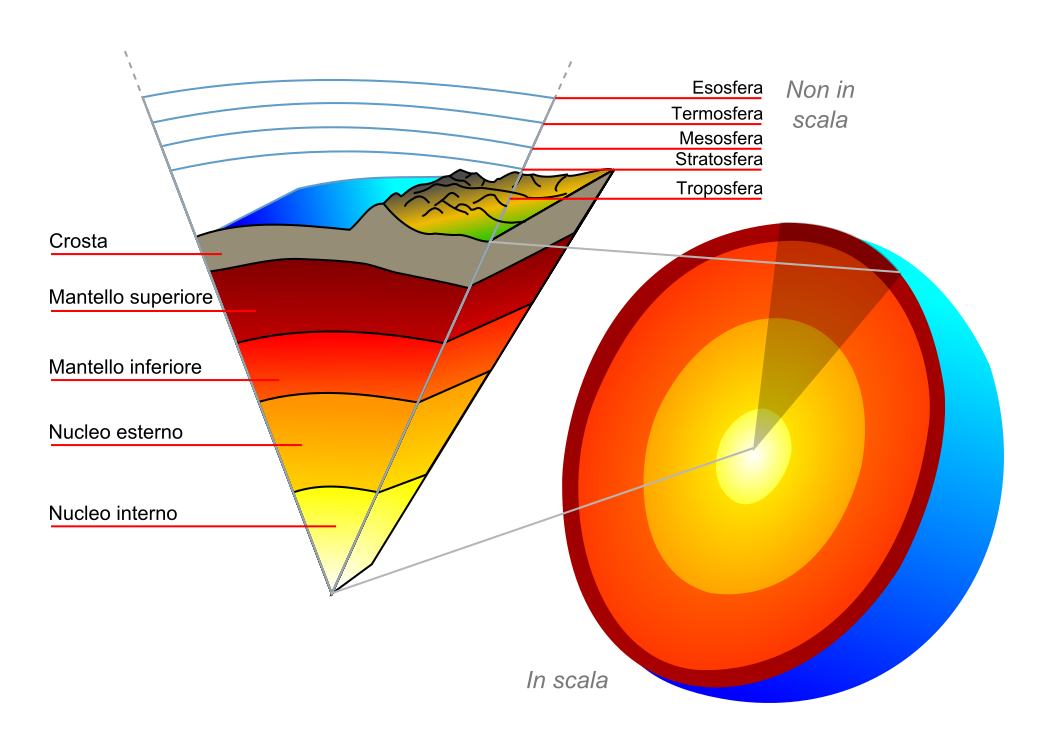
\includegraphics[width=0.50\textwidth]{Chapter-1/crosta-terrestre.png}
\end{wrapfigure}

La terra è composta a strati, o meglio da involucri concentrici (Figura \ref{fig:crostaterrestre}) ed ognuno di essi ha diverse caratteristiche e particolarità.
Al centro della Terra c'è il \textbf{nucleo interno}, ossia un ammasso viscoso composto quasi esclusivamente da ferro avente un raggio di circa 1250 km. Si raggiungono temperature molto elevate, circa 5000-6000$^{\circ}$C.
A seguire abbiamo il \textbf{nucleo esterno}, principalmente composto per il 20\% da ferro e la restante parte nichel, raggiunge circa i 3000$^{\circ}$C. Comprendendo anche il nucleo interno, ha un raggio di circa 3500 km.

Continuando verso l'esterno, troviamo il \textbf{mantello terrestre}, che si divide in superiore ed inferiore.
\\
È composto da diversi metalli ed è difficile stabilire la temperatura dato i moti convettivi del calore, ma si stima intorno ai 500$^{\circ}$C a confine con la crosta terrestre e 3000$^{\circ}$C a confine con il nucleo.
Infine abbiamo la \textbf{crosta terrestre}, che partendo dalla superficie, arriva fino a 70 km di profondità.
Insieme, il \textit{mantello superiore} e la \textit{crosta terrestre} formano la \textbf{litosfera}.
La litosfera è suddivisa in una decina di placche tettoniche principali e altre numerose placche di minori dimensioni (figura \ref{fig:placchetettoniche}). Queste placche ``galleggiano" sullo strato immediatamente sottostante del mantello superiore.\cite{terra}

Esse, data la forte pressione e le alte temperature, subiscono sforzi di enormi dimensioni che formano i \textbf{terremoti}.
I terremoti sono vibrazioni della crosta terrestre, provocate dallo spostamento  di una o più placche nella litosfera.
Le placche si muovono flettendosi lentamente e poi rilasciando (raggiunto il \textit{punto di rottura}) in maniera elastica tutta l'energia accumulata.
Il punto in cui viene generata questa energia è detto \textbf{ipocentro} (2), zona in cui è presente una frattura chiamata \textit{faglia} (3), mentre il punto in superficie posto sulla verticale dell'ipocentro è chiamato \textbf{epicentro} (1).
\begin{figure}[ht]
\label{fig:ipocentro}
\centering
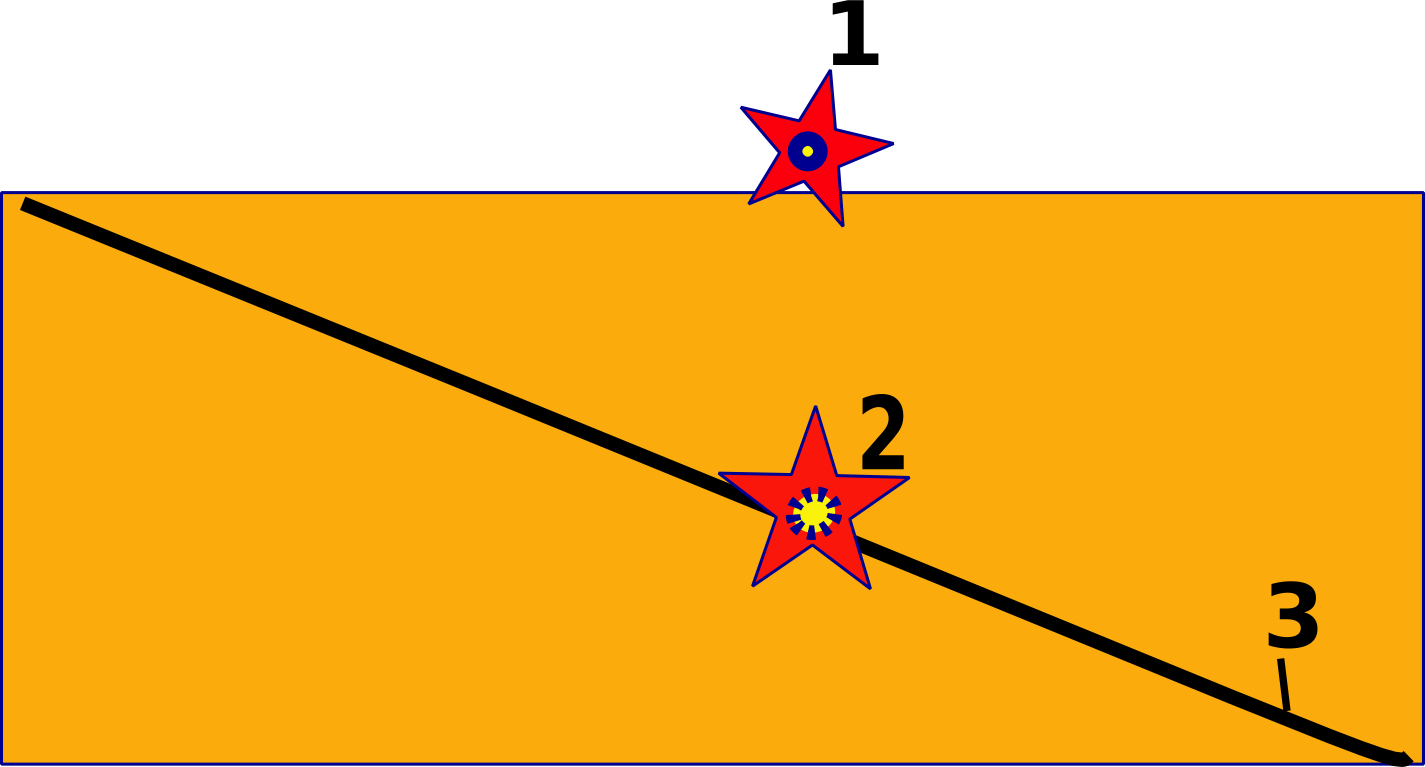
\includegraphics[width=0.55\textwidth]{relazione-tirocinio/Chapter-1/ipo-epi-centro.png}
\end{figure}

\clearpage

\begin{figure}
\caption{Placche tettoniche}
\label{fig:placchetettoniche}
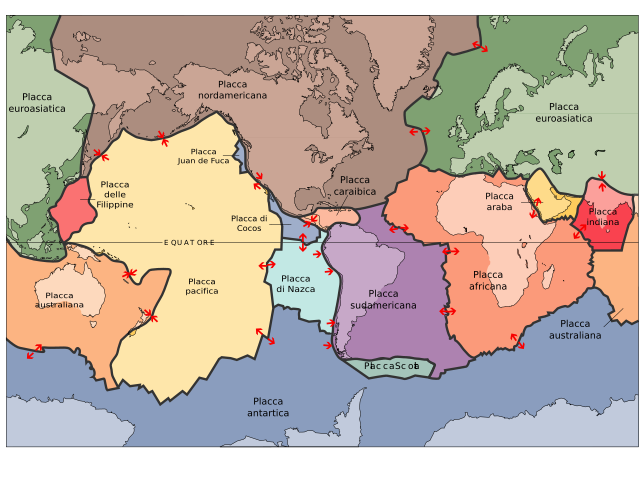
\includegraphics[width=1\textwidth]{Chapter-1/placche-tettoniche.png}
\end{figure}
Esistono tre tipi di faglie: faglie \textit{trascorrenti}, faglie \textit{dirette} e \textit{inverse}.
Esistono in egual numero differenti tipi di onde sismiche.
\\
Le \textbf{onde di compressione o longitudinali} fanno comprimere e dilatare la materia nella stessa direzione con cui si propaga l'onda.
Sono anche dette \textit{primarie}, perché sono le onde che viaggiano a velocità più elevate.
\\
Le \textbf{onde di taglio o trasversali} fanno compiere alla materia oscillazioni in modo perpendicolare alla loro direzione di propagazione. Hanno effetto solo nei solidi, non possono propagarsi attraverso corpi liquidi o gassosi.
Vengono chiamate anche \textit{onde secondarie}, essendo meno veloci delle precedenti.
\\
Le \textbf{onde superficiali}, anche se il nome può essere mal interpretato, non si manifestano in superficie. Questo tipo di onde sono la combinazione delle due precedenti, perciò sono molto complesse e sono le più pericolose. 

\clearpage

\section{Misurazione dei terremoti}

\subsection{Tipologie di terremoti}
Esistono 4 differenti tipologie di terremoti: \textit{tettonici}, \textit{vulcanici}, \textit{da crollo} e \textit{artificiali}.
\\
I terremoti \textbf{tettonici}, come dice il nome, sono provocati dal movimento delle placche tettoniche e hanno origine lungo le faglie.
Sono i più pericolosi ed i più frequenti.
\\
I terremoti \textbf{vulcanici} sono originati dall'attività vulcanica nel sottosuolo. Sono meno pericolosi dei precedenti data la minor energia rilasciata e l'estensione limitata.
\\
I terremoti \textbf{da crollo} si originano durante il crollo di montagne, grotte o frane. Hanno una bassa pericolosità e frequenza.
\\
Infine, i terremoti \textbf{artificiali} vengono originati da attività umane. Ad esempio, una grande esplosione. In generale, hanno una potenza molto limitata.

\subsection{Metodologie di misurazione}
Esistono due tipologie principali di misurazione di un terremoto: la scala \textbf{Mercalli} e la scala \textbf{Richter}.
La scala Mercalli misura l'\textit{intensità} di un terremoto osservando i danni causati da esso. Per questo, dato che tiene in conto solo degli effetti che la scossa produce, può essere applicata anche ai terremoti avvenuti nel passato.
Assegna dei numeri crescenti per intensità, si va dall'uno (impercettebile) sino a dodici (apocalittica).
La scala (o meglio \textit{indice}) Richter misura invece l'energia sprigionata dalla scossa, ossia la \textit{magnitudo}. Viene chiamata scala, ma è più corretto dire indice dato che non ha un range di valori finito. La magnitudo è descritta da questa formula:
\begin{equation*}
  M_w = {\frac{2}{3}}\log_{10}(M_\mathrm{0}) - 10,7
\end{equation*}
dove $M_0$ è il momento sismico all'ipocentro da esprimere in Newton per metro|N·m.\cite{measure}
Ad oggi il massimo valore magnitudo registrato è 9,5.

\subsection{Strumenti di misurazione}
Sono principalmente due: il \textbf{sismografo} ed il \textbf{sismometro}.
Entrambi misurano accelerazione e velocità dei movimenti del suolo, con la differenza che il sismometro misura solamente, ma non può registrare i dati; il sismografo invece oltre alla misura produce anche un grafico temporale, chiamato appunto \textit{sismogramma}.
Uno strumento non può misurare ampie porzioni di territorio, per questo si creano delle reti che monitorano degli ampi spazi di suolo. In Italia questa rete è la \textbf{Rete Sismica Nazionale}.
Con le tecnologie odierne, si utilizzano sismometri digitali insieme ad altri strumenti. Ad esempio, nella rete italiana, le stazioni sono composte da un sismometro, un accelerometro ed una antenna e ricevitore GPS.
È una rete di stazioni sismiche (circa 300) disposte su tutto il territorio italiano e appena fuori dai confini.
Per la maggioranza sono stazioni dell'INGV (Istituto Nazionale di Geologia e Vulcanologia), ma ne fanno parte anche altre piccole reti.
Questa rete monitora sette giorni su sette, 24 ore su 24 i movimenti del suolo e li registra, inviandoli poi ai centri di elaborazione dati di Roma, Grottaminarda e Catania.
La concentrazione maggiore di terremoti in Italia è nell'appennino e nel sud Italia, per questo la maggior parte delle stazioni è posizionata in questi punti, come si può notare nella Figura \ref{fig:RSN}.

\clearpage

\begin{figure}
\caption{Rete Sismica Nazionale \cite{ingv}}
\label{fig:RSN}
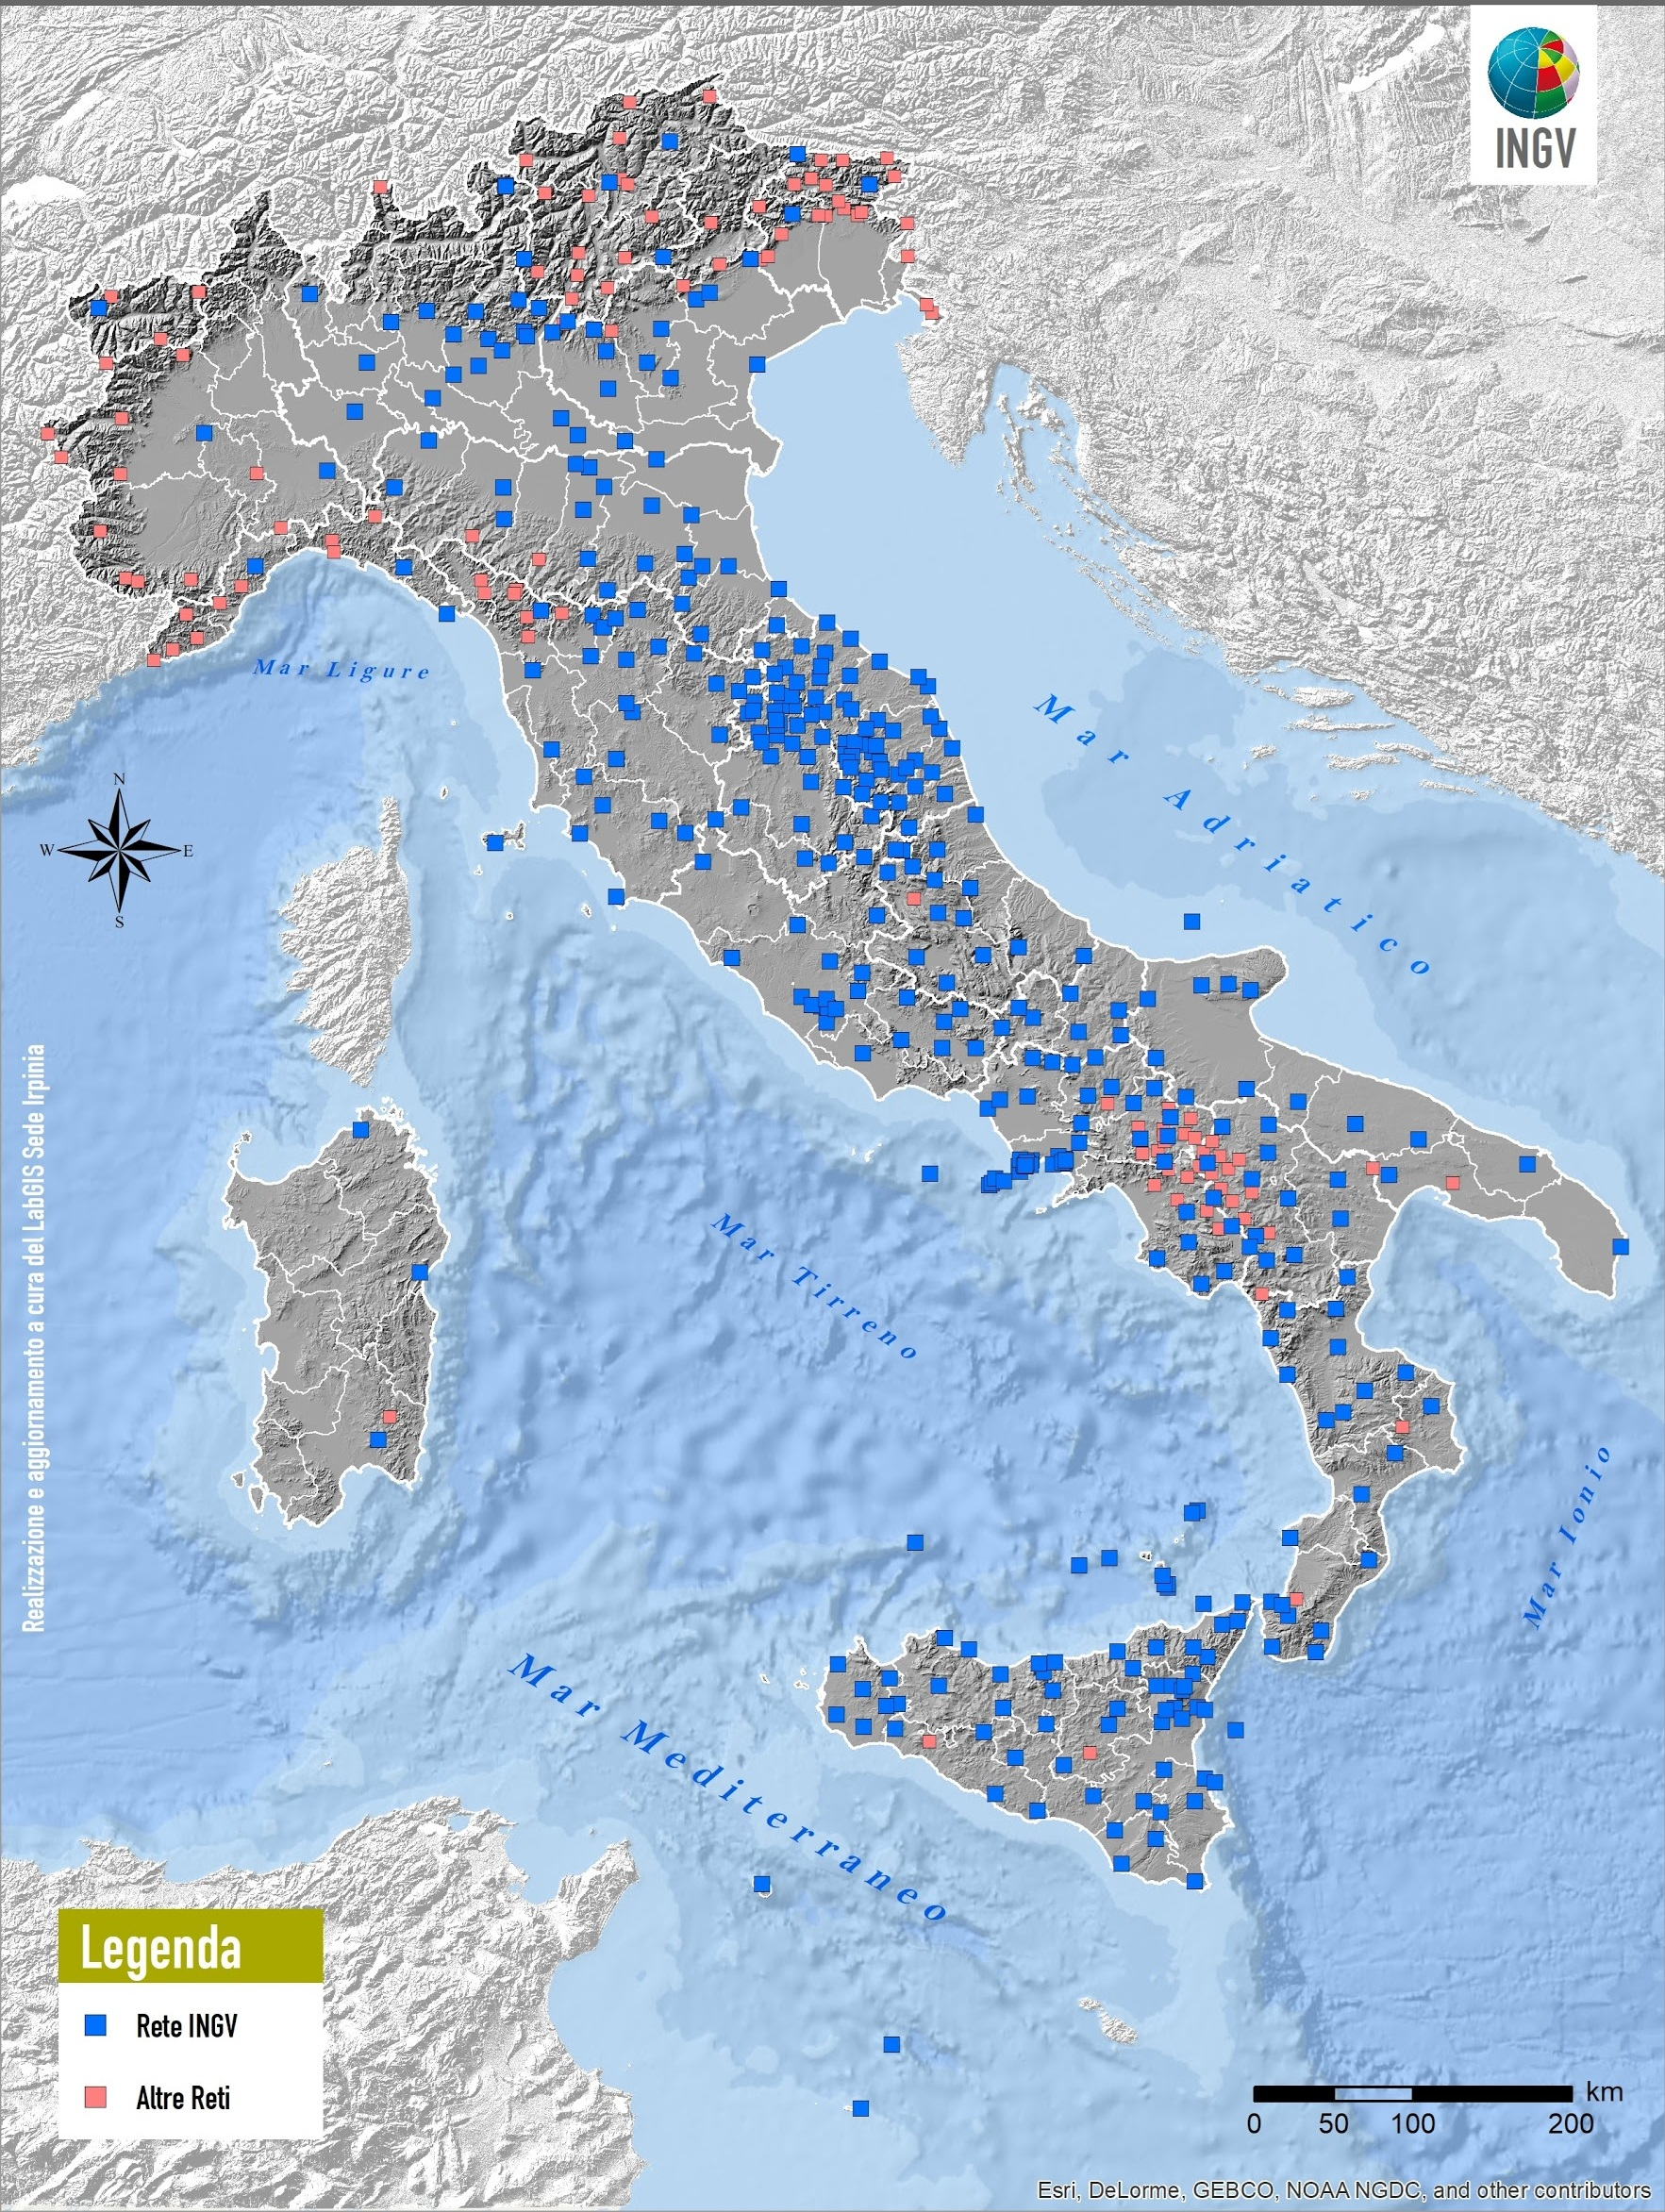
\includegraphics[width=1\textwidth]{Chapter-1/RSN.jpg}
\end{figure}

\clearpage

\section{Piattaforma SeismoCloud}

\subsection{Introduzione al progetto}

\begin{wrapfigure}[14]{r}{0.15\textwidth}

\includegraphics[width=0.15\textwidth]{Chapter-1/seismocloud.png}

\includegraphics[width=0.15\textwidth]{Chapter-1/ingv.jpg}
\end{wrapfigure}

SeismoCloud è una rete di dispositivi IoT (Internet of Things) a basso costo connessi fra loro distribuiti in tutta Italia.
Ha come scopo l'\textbf{Earthquake Early Warning}, ossia monitorare l'attività sismica e, nel caso viene rilevato un terremoto, notificare le persone interessate.
L'obiettivo specifico dell'EEW è l'avviso \textbf{in tempo reale} di un possibile sisma.
I sismometri possono essere costruiti personalmente se si ha capacità di elettronica di base, altrimenti viene utilizzato il sensore interno di uno smartphone.
Come si può notare dalla Figura \ref{fig:RSS} la \textbf{Rete Sismica SeismoCloud} si estende su tutto il territorio nazionale. Si contano circa 100 sismometri attivi.
Ad oggi il sistema EEW non è attivo perché i sismometri presenti non bastano a compiere delle rilevazioni sufficienti a stabilire l'effettiva presenza di un sisma.
I nodi della rete sono ben distribuiti nel nord e centro Italia, male nel Sud. Questo è un problema perché l'attività sismica principale italiana si sviluppa lungo la catena appenninica fino in Sicilia.
Grande menzione meritano anche i vulcani attivi (Etna, Stromboli, Vesuvio, Vulcano).
È un progetto nato dall'Università La Sapienza e l'INGV. Viene presentato anche nelle scuole per sensibilizzare gli studenti sul tema terremoti ed
utilizzare questo progetto come
strumento didattico.
Il codice di alcune porzioni di sistema è disponibile su GitHub sotto
l'organizzazione \href{https://github.com/SapienzaApps}{SapienzaApps}.

\begin{figure}[ht]
\centering
\caption{Rete Sismica SeismoCloud}
\label{fig:RSS}
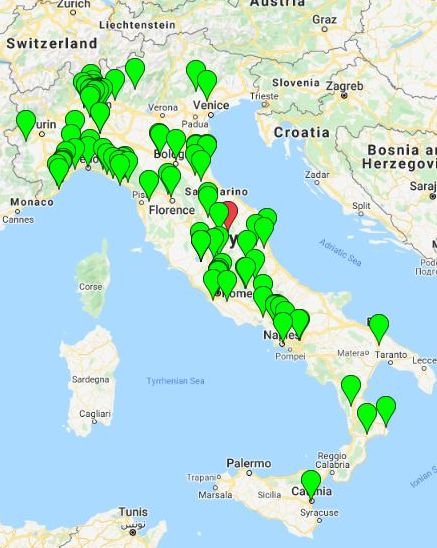
\includegraphics[width=0.55\textwidth]{Chapter-1/seismoitalia.jpg}
\end{figure}

\subsection{Architettura di sistema}
I sismometri sono di due tipologie: \textit{fissi} e \textit{mobili}.
I \textbf{sismometri fissi} sono dei moduli formati da componenti elettronici a basso costo. Viene usato un chip con un modulo Wi-Fi integrato per la connessione ad Internet, nello specifico il NodeMCU/ESP8266 e un modulo con giroscopio e accelerometro, l'MPU6050.
Sono pensati per essere fissati a muri portanti per una migliore rilevazione.
I \textbf{sismometri mobili} invece utilizzano l'applicazione per smartphone, abilitando l'accelerometro interno del telefono per rilevare vibrazioni.
Devono essere appoggiati su un piano orizzontale, per esempio un tavolo, per avere una rilevazione precisa.
Durante la registrazione di un nuovo sismometro fisso esso viene localizzato per conoscere la sua posizione (fondamentale al rilevamento corretto dei sismi), mentre i sismometri mobili aggiornano di continuano la loro posizione. Nonostante ciò la privacy può essere conservata mostrando il sismometro nella mappa pubblica con una finta posizione casuale nel raggio di 2km.
I sismometri utilizzano il protocollo ISO standard \textbf{MQTT} (Message Queue Telemetry Transport) per inviare e ricevere messaggi di controllo e dati.

\begin{figure}[ht]
\centering
\label{fig:mqtt}
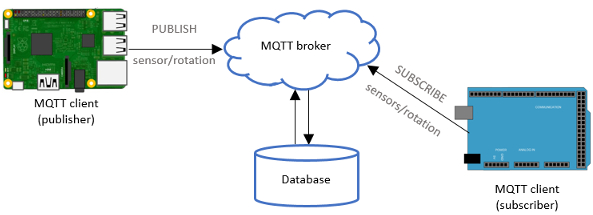
\includegraphics[width=1\textwidth]{Chapter-1/mqtt.jpg}
\end{figure}
Viene utilizzato questo protocollo perché è stato progettato per i dispositivi IoT, dato che questi ultimi hanno, solitamente, una batteria con piccola capienza ed in generale risorse limitate. Rispetto al precedente protocollo HTTP, esso invia messaggi ad alta affidabilità, ha una bassa latenza ed un basso overhead\cite{ottimizzazione}. In MQTT, il \texttt{topic} è una stringa UTF-8 che un broker utilizza per filtrare i messaggi. 
Si può considerare come una etichetta che viene affissa a dei valori che si riferiscono tutti allo stesso argomento. Un broker è il responsabile della comunicazione tra i vari client connessi. I topic hanno una gerarchia basata a livelli ed ogni livello è separato da uno slash. 
Ad esempio il topic che si riferisce alla temperatura del sismometro con identificativo $34$ potrebbe essere \texttt{sensor/34/temperature}.
Dato che MQTT è un protocollo di tipo \textit{publish/subscribe}, i client possono pubblicare dati relativi ad un topic, i quali verranno ricevuti dai client che sono iscritti a quel determinato topic.
I client sono liberi di scegliere le azioni da compiere: possono solamente iscriversi ad alcuni topic (o a tutti), oppure solamente pubblicare dati su topic senza iscriversi, oppure possono eseguire entrambe le operazioni.
I dati inviati vengono poi elaborati in un server centrale che li gestisce, compie dei calcoli su di essi (allo scopo di identificare una possibile scossa di terremoto e attivare una notifica di Earthquake Early Warning) e li archivia in un database. 

\clearpage

Quando gli utenti richiedono i dati (da app o interfaccia web) non viene utilizzato il protocollo MQTT, ma il protocollo HTTP (Hyper Text Transfer Protocol).
Per i messaggi inviati tramite HTTP viene utilizzato lo stile architetturale \textbf{REST} (REpresentational State Transfer).
Questo schema è definito da dei principi \cite{rest}:
\begin{itemize}
  \item \texttt{Client-Server}: Separare l'interfaccia dalla logica dei dati aumenta la portabilità del sistema.
  \item \texttt{Stateless}: Ogni richiesta dal client al server non deve basarsi su altri dati se non quelli interni alla richiesta.
  \item \texttt{Cacheable}: I dati, se possibile, devono essere salvati nella cache del client per utilizzi futuri.
  \item \texttt{Interfacce uniformi}: Prediligere identificazione delle risorse; manipolazione delle risorse tramite rappresentazioni; messaggi auto-esplicativi; hypermedia come motore dello stato dell'applicazione.
  \item \texttt{Sistema a livelli}: un sistema composto da più livelli indipendenti rende il sistema modulare.
  \item \texttt{Codice su richiesta (opzionale)}: È permesso scaricare ed eseguire codice (applet o script) per snellire il client.
\end{itemize}
Il nucleo dello stile REST sono le \textit{risorse}.
Una risorsa è qualsiasi informazione: un documento, una immagine, un video, un numero, una collezione di risorse.
REST utilizza identificatori di risorse per aiutare la comunicazione tra le parti.
Un esempio di risorsa in stile REST è: \texttt{example.domain/sensor/sensor-id/quake}, dove \texttt{sensor-id} è l'identificatore unico per un sensore.
Tramite l'app mobile (disponibile per Android e iOS) si registrano i nuovi sismometri (sia fissi che mobili). Il sismometro interno viene registrato automaticamente quando viene scaricata l'applicazione per la prima volta. Il sismometro fisso invece crea una connessione Wi-Fi chiamata \textit{SeismoCloud}. L'utente ci si collega ed inserisce i dati per connettersi alla rete Wi-Fi locale. Successivamente in automatico il dispositivo fisso si collega alla rete Wi-Fi e l'app cerca di trovare nella rete un sismometro.
In entrambi i casi viene richiesto di consentire all'acquisizione della posizione GPS ed un nome per il nuovo sismometro.
Attivando un sismometro viene prodotta una mole consistente di dati.
\begin{center}
Esempio di dati ricevuti e/o inviati dal dispositivo
\end{center}
\begin{lstlisting}[numbers=none]
timereq = 1597913685108
timesync = 1597913685108;1597913683476;15979136857668
publicip = 129.65.2.45
localip = 192.168.0.12
essid = wifi-locale
rssi = -58.744674356
bssid = aa:bb:cc:dd:ee:ff
treshold = 27200000.0000
temperature = 34.100000
quake = 1597913685178;0.644563;0.353425;0.683452
location = 40.857634274356;15.24525254252
\end{lstlisting}
Con una cadenza periodica (qualche minuto, dipende dal carico del sistema) vengono pubblicati: indirizzo IP locale e pubblico, indirizzo MAC e qualità del segnale della rete Wi-Fi, localizzazione e temperatura del sismometro, soglia attuale (valore utile alla rilevazione di una vibrazione).
Quando il sismometro rileva una vibrazione viene inviata l'intensità della vibrazione.
Un topic MQTT è dedicato al comando \textit{reboot}, ossia la possibilità di riavviare il sismometro pubblicando un messaggio.\\
Inoltre è possibile visualizzare la lista dei propri sismometri, una mappa aggiornata in tempo reale con i sismometri attivi e i terremoti recenti, una lista di terremoti con relativa magnitudo, posizione e profondità dell'ipocentro (ordinati cronologicamente) e infine alcuni informazioni utili.
È disponibile anche una interfaccia web dove è possibile visualizzare tutte le informazioni prima citate ed in più una dashboard personalizzata.
In quest'ultima è possibile visualizzare due grafici che mostrano il tempo di utilizzo assoluto e settimanale di ogni sismometro attivo.
Dopo l'effettiva autenticazione (tramite password o QRCode) si entra nell'area privata, ossia relativa ad un determinato \textit{gruppo} (insiemi di sismometri raggruppati per locazione).
Qui, oltre alle funzionalità citate, è presente un sistema di \textbf{EUD} (End User Development).
Dalla pagina Wikipedia \cite{wikieud}:
\begin{quoting}[font=itshape, begintext={``}, endtext={``}]
Lo sviluppo per l'utente finale (EUD) o la programmazione per l'utente finale (EUP) si riferisce ad attività e strumenti che consentono agli utenti finali, persone che non sono sviluppatori di software professionisti, di programmare i computer. Le persone che non sono sviluppatori professionisti possono utilizzare gli strumenti EUD per creare o modificare artefatti software (descrizioni di comportamenti automatizzati) e oggetti di dati complessi senza una conoscenza significativa di un linguaggio di programmazione.
\end{quoting}
Ad esempio, si può ricevere un messaggio automatico tramite Telegram ogni volta che il mio sismometro vibra. Questo sistema viene spiegato meglio nel paragrafo 3.1 Sistema Legacy.

\begin{figure}
\caption{Architettura di SeismoCloud}
\label{fig:ArchitetturaSeismoCloud}
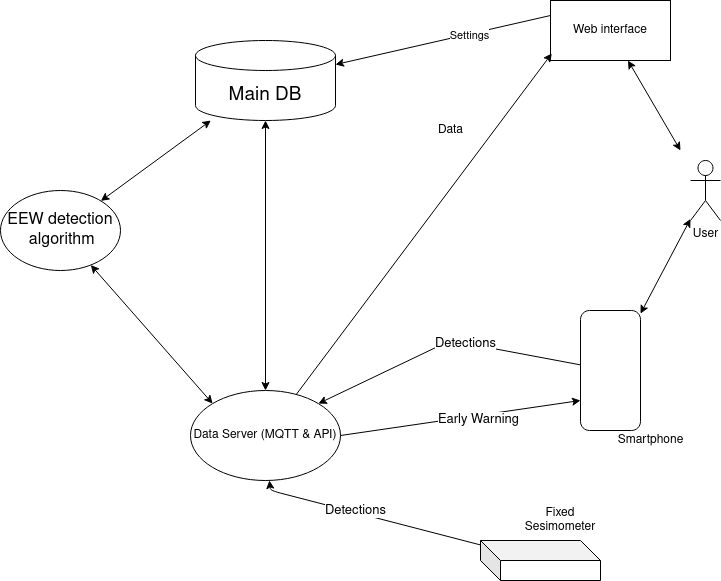
\includegraphics[width=1\textwidth]{Chapter-1/architettura-seismocloud.png}
\end{figure}

\clearpage

% ======================================= CHAPTER 2 ================================================
\chapter{Progettazione dell'architettura del sistema EUD}

\section{Scelta dello strumento di sviluppo}

\subsection{Candidati iniziali}

Piuttosto che progettare e costruire uno strumento di End User Development da zero, si è cercato uno scheletro già pronto e maturo. La ricerca è stata piuttosto semplice, un po' meno la valutazione dei possibili candidati.
Il primo candidato è \textbf{IFTTT} (\href{https://iftt.com}{https://ifttt.com}). È lo strumento più famoso, utilizzato da molte persone, con più di 5 milioni di download su Play Store. Il vantaggio di questa scelta è sicuramente la grande maturità della piattaforma. Gli svantaggi sono la difficoltà nell'integrare i nostri dispositivi con questo sistema, ma soprattutto la somiglianza con il sistema EUD da rimpiazzare, troppo semplice e con condizioni e azioni predefinite.
Una seconda scelta è \textbf{draw.io} (\href{https://app.diagrams.net/}{https://draw.io}). Strumento completamente differente al precedente, è un creatore di diagrammi di flusso. Questo è un tipo di programmazione di azioni che lascia molta libertà all'utente, rimanendo semplice ma efficace. 
\begin{figure}[H]
\caption{Esempio di flusso esportato da draw.io}
\label{fig:drawio}
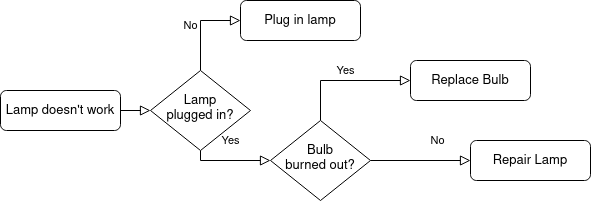
\includegraphics[width=1\textwidth]{relazione-tirocinio/Chapter-2/drawio.png}
\end{figure}
Il codice sorgente di draw.io è disponibile su GitHub. È  ben documentato, quindi questo aiuta l'integrazione con SeismoCloud. Purtroppo si tratta di uno strumento front-end, quindi manca tutta la logica back-end; i dati inseriti dall'utente vengono esportati in file di tipo xml che devono poi essere tradotti in azioni registrate dal sistema. 

\subsection{La piattaforma Node-RED}
Lo strumento che risolve i problemi precedentemente elencati è \textbf{Node-RED} (\href{https://nodered.org}{https://nodered.org}).
Come draw.io è un creatore di diagrammi di flusso ed è anche open-source con repository su GitHub sotto l'organizzazione \href{https://github.com/node-red}{node-red}. È un servizio orientato all'\textit{Internet of Things}, non è uno standard ufficiale, ma è molto utilizzato nel campo.
A differenza del precedente esiste uno scheletro back-end, dato che è costruito utilizzando \href{https://nodejs.org}{NodeJS}. Vedremo più avanti in dettaglio come è stato progettato.
La community, oltre ad essere pronta a risolvere dubbi sul forum ufficiale (\href{https://discourse.nodered.org}{discourse.nodered.org}), contribuisce attivamente al progetto implementando delle funzionalità che sono messe a disposizione di tutti tramite il famoso package manager NPM.
Nel nome il `node' è dato sia dal runtime NodeJS, sia dal nome che hanno gli elementi utilizzati per creare i flussi, chiamati appunto \textit{nodi}.
\begin{figure}[H]
\caption{Esempio flusso di nodi in Node-RED}
\label{fig:node-red-flows-example1}
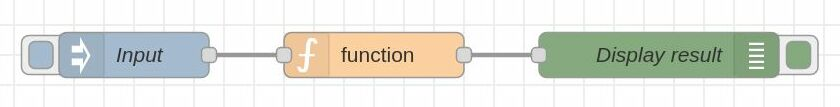
\includegraphics[width=1\textwidth]{relazione-tirocinio/Chapter-2/node-red-flows-1.jpg}
\end{figure}
Come si nota in figura \ref{fig:node-red-flows-example1}, i nodi sono dei rettangoli che hanno funzioni particolari:
\begin{itemize}
    \item \textbf{Nodi input}: Questi nodi emettono valori e non prendono nulla in ingresso, quindi sono utilizzati per produrre dati o iniziare dei flussi. Possono avere da 1 a n valori in uscita.
    \item \textbf{Nodi intermedi}: Sono nodi che hanno sia input che output. Sono utilizzati per applicare delle funzioni ai dati in ingresso, oppure il dato in ingresso viene solamente utilizzato per far iniziare una procedura intermedia. Prendono in input un solo valore e possono avere da $1$ a $n$ valori in uscita.
    \item \textbf{Nodi output}: Sono gli opposti dei nodi input. Non hanno valori in uscita ma solo in ingresso. Sono utilizzati per terminare un flusso, solitamente sono quindi le azioni da effettuare nel caso in cui si verificano le condizioni stabilite. Possono avere un solo valore in ingresso.
\end{itemize}
\begin{figure}[H]
\caption{Esecuzione del comando shutdown}
\label{fig:node-red-flows-example2}
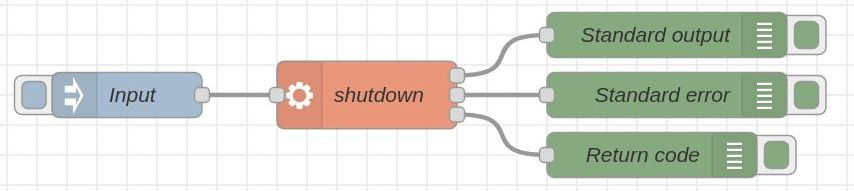
\includegraphics[width=1\textwidth]{relazione-tirocinio/Chapter-2/node-red-flows-2.jpg}
\end{figure}
Nella figura \ref{fig:node-red-flows-example2} abbiamo un altro esempio. Qui quando viene cliccato il pulsante a sinistra del nodo \textit{input}, il nodo invia in uscita un valore (in questo caso qualsiasi, ad esempio 3 o la stringa 'input') che fa eseguire il secondo nodo (di tipo \textit{intermedio}). Il nodo \textit{shutdown} esegue il comando `shutdown` e stampa nella console di debug lo stdout, stderr ed il return code.
Data la facilità d'uso, il grande supporto (repository con 10+K star su GitHub, community molto attiva e forum ufficiale), la maturità del progetto (versione 0.2 nel 2013, ad oggi (2020) 1.1.3), la facile estendibilità ed integrazione con dispositivi IoT (come appunto i nostri sismometri), decisamente Node-RED è lo strumento più adatto per risolvere i bisogni della community SeismoCloud.

\clearpage

\section{Architettura adattata a SeismoCloud}

\subsection{Come funziona Node-RED}
Può essere utilizzato in vari modi, ad esempio: su un computer in locale, tramite Docker, su un dispositivo Raspberry, oppure su alcuni sistemi Cloud (IBM Cloud, Amazon Web Services, Microsoft Azure).
L'interazione con l'utente avviene completamente tramite un browser web. Viene fornita una pagina divisa in tre sezioni: un insieme di funzionalità (nodi) disponibili, un foglio di lavoro dove poter creare i vari flussi ed un modulo di aiuto, documentazione e debug.
Un \textbf{nodo} è il blocco costruttivo di base di un flusso. Le funzionalità dei nodi sono scatenate da eventi esterni (richieste HTTP o altro protocollo oppure un timer) o da input ricevuti da altri nodi. Processano il messaggio ricevuto oppure ne creano uno nuovo e possono inviare messaggi ai nodi successivi nel flusso. 
Un \textbf{nodo di configurazione} è un tipo speciale di nodo che setta delle configurazioni utili agli altri nodi, ma non fa parte di nessun flusso. Ad esempio, i nodi \textit{MQTT-in} e \textit{MQTT-out} utilizzano il nodo di configurazione \textit{MQTT-broker} che rappresenta una connessione condivisa con un broker MQTT.
Un \textbf{flusso} è rappresentato da un tab o foglio di lavoro ed è il metodo principale per organizzare il lavoro. Informalmente un flusso rappresenta un insieme di nodi connessi fra loro.
Un \textbf{sottoflusso} è una collezione di nodi che vengono collassati graficamente in un unico nodo. Possono essere utilizzati per ridurre la complessità grafica del flusso, oppure per riutilizzare un gruppo di nodi più volte in un flusso.
\begin{figure}[H]
\caption{Esempio di sottoflusso}
\label{fig:sottoflusso}
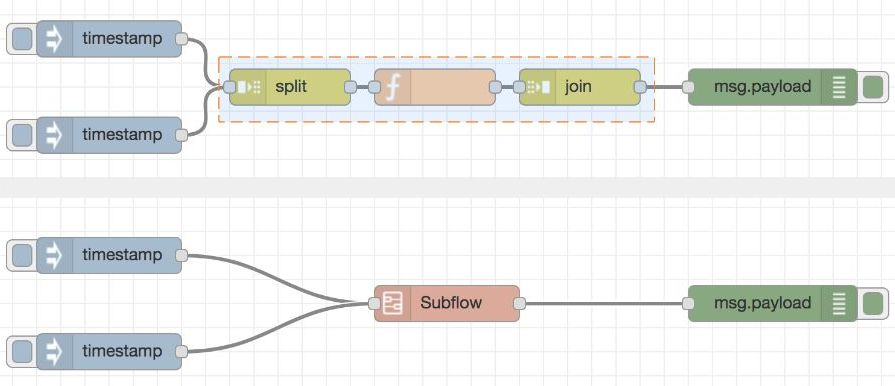
\includegraphics[width=1\textwidth]{relazione-tirocinio/Chapter-2/node-red-flows-4.jpg}
\end{figure}
Il \textbf{contesto} è il modo principale di condividere informazioni tra i nodi senza essere connessi fra loro. Ne esistono di tre tipi:
\begin{itemize}
    \item Node: Visibile solamente dal nodo che setta il valore
    \item Flow: Visibile a tutti i nodi che appartengono allo stesso flusso (o tab)
    \item Global: Visibile a tutti i nodi
\end{itemize}
Un \textbf{messaggio} è un oggetto JSON che viene passato attraverso i nodi. Di default si chiama \textit{msg} ed ha due campi: \textit{payload} e \textit{id}. 
La \textbf{palette} è posizionata sulla sinistra dell'interfaccia e lista tutti i nodi presenti nel sistema. Dei nodi extra possono essere aggiunti direttamente dall'editor.
Il \textbf{workspace} è lo spazio principale, dove tutti i nodi vengono posizionati in modo da creare degli automatismi.
La \textbf{sidebar} è uno spazio posizionato a destra del workspace in cui ci sono degli strumenti utili, ad esempio la console di debug, l'interfaccia della configurazione dei nodi e la finestra descrittiva per ogni nodo.
È molto orientato al riuso ed alla portabilità, infatti tutti i nodi o collezioni di nodi sono moduli Javascript che possono essere caricati e utilizzati poi da altre persone tramite NPM.
Inoltre, ogni flusso viene poi tradotto in codice JSON per poter essere esportato ed importato in altri ambienti.
Viene fornita anche una `vetrina' (\href{https://flows.nodered.org}{flows.nodered.org}) dove possono essere esplorati nodi e flussi creati e pubblicati per la community.
Esempio di un semplice flusso Node-RED:
\begin{figure}[H]
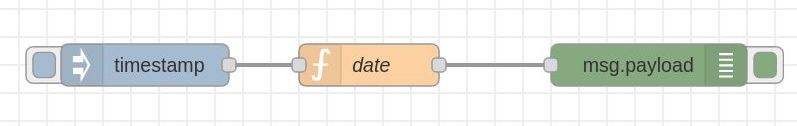
\includegraphics[width=1\textwidth]{relazione-tirocinio/Chapter-2/node-red-flows-3.jpg}
\end{figure}
Il nodo \textit{date} non è altro che un nodo function che restituisce la data:
\begin{lstlisting}[language=JavaScript]
// Create a Date object from the payload
var date = new Date(msg.payload);
// Change the payload to be a formatted Date string
msg.payload = date.toString();
// Return the message so it can be sent on
return msg;
\end{lstlisting}
Viene tradotto così in JSON:
\begin{lstlisting}[language=JavaScript]
[
    {
        "id":"58ffae9d.a7005",
        "type":"debug",
        "name":"",
        "active":true,
        "complete":false,
        "x":640,"y":200,
        "wires":[]
    },
    {
        "id":"17626462.e89d9c",
        "type":"inject",
        "name":"timestamp",
        "topic":"",
        "payload":"",
        "repeat":"",
        "once":false,
        "x":240,
        "y":200,
        "wires":[["2921667d.d6de9a"]]
    },
    {
        "id":"2921667d.d6de9a",
        "type":"function",
        "name":"date",
        "func":"// Create a Date object from the payload\nvar date = new Date(msg.payload);\n// Change the payload to be a formatted Date string\nmsg.payload = date.toString();\n// Return the message so it can be sent on\nreturn msg;",
        "outputs":1,
        "x":440,
        "y":200,
        "wires":[["58ffae9d.a7005"]]
    }
]
\end{lstlisting}
Dato che Node-RED ha tutti i dati in-memory, per salvare i flussi creati utilizza (di default) un file chiamato \textit{flows.json}. Questo rende molto facile condividere i progetti.

\subsection{Requisiti di sistema}
Una caratteristica del precedente sistema che viene riportata nel nuovo è la divisione netta dei dati dei vari gruppi e la condivisione di essi nel gruppo di appartenenza.
Questa scelta consente agli utenti di avere a disposizione più dati rispetto a quelli che avrebbero utilizzando solo i propri dispositivi. In media un utente ha un solo dispositivo proprietario, mentre un gruppo ne ha tra i dieci ed i quindici.
Questo consente agli utenti di avere \textbf{ampia libertà nella scelta delle condizioni}.
Quindi un requisito fondamentale è la \textit{scissione e la replica di un sistema in più "copie" con dati differenti} (i gruppi in questo caso).
I requisiti non funzionali che devono essere rispettati sono:

\begin{itemize}
    \item Funzionalità: Devono essere garantite le funzionalità presenti nel precedente sistema ed in più ampliare dove possibile con le richieste (valutate dal team di sviluppo) degli utenti.
    \item Usabilità: Il sistema deve risultare semplice e utilizzabile ad un pubblico più vasto possibile. Verrà testata l'usabilità con varie tipologie di test.
    \item Affidabilità: Deve essere garantita la sicurezza dei dati e la privacy degli utenti. Il sistema deve essere costruito seguendo \textit{privacy by design}.
    \item Prestazioni: Il sistema non deve sprecare risorse (sia di memoria, sia computazionali) e deve essere progettato con molta attenzione alle performance. 
\end{itemize}
L'usabilità verrà discussa nel capitolo 3 e nel capitolo 5,
l'affidabilità nel capitolo 4.

\clearpage


\subsection{Vantaggi nell'utilizzo di Docker}

Lo strumento che più soddisfa i requisiti imposti è \textbf{Docker}.
È uno dei sistemi più noti per il deployment di applicazioni software. Dalla pagina Wikipedia che descrive Docker
\cite{wikidocker}:
\begin{quoting}[font=itshape, begintext={``}, endtext={``}]
Docker è un progetto open-source che automatizza il deployment (consegna o rilascio al cliente, con relativa installazione e messa in funzione o esercizio, di un'applicazione o di un sistema software tipicamente all'interno di un sistema informatico aziendale) di applicazioni all'interno di contenitori software, fornendo un'astrazione aggiuntiva grazie alla virtualizzazione a livello di sistema operativo di Linux. Docker utilizza le funzionalità di isolamento delle risorse del kernel Linux come ad esempio cgroup e namespace per consentire a "container" indipendenti di coesistere sulla stessa istanza di Linux, evitando l'installazione e la manutenzione di una macchina virtuale.
\end{quoting}

Il concetto di container è già disponibile in Linux per eseguire un processo su cui possono essere limitate e gestite le risorse a lui allocate. Il problema dei container LXC (disponibili in Linux utilizzando cgroup e namespace) è che se un container viene spostato su una macchina con configurazione differente è molto probabile che non funziona, dato che ogni container dipende dall'ambiente in cui è costruito (dipendenze esterne, configurazione di rete, memoria e
impostazioni aggiuntive). Docker aggiunge \textbf{portabilità} ai container, cioè utilizzando un motore Docker i container diventano indipendenti dalla macchina in cui è stato creato. Altra funzione aggiunta è il \textbf{versioning}; si può tenere traccia delle varie versioni di un container, dando la possibilità di un upgrade o downgrade. Inoltre è orientato al \textbf{riuso},     dato che ogni container può essere utilizzato come base per uno più specifico \cite{docker-portability}.
Docker definisce un formato unico per creare container, più nello specifico \textit{immagini}. Una immagine è il risultato dell'esecuzione di un file chiamato \textbf{Dockerfile}. Viene fornito il DockerHub, un portale dove sono presenti migliaia di immagini già pronte che possono essere utilizzate come base di partenza.

\vspace{0.02\textwidth}
\begin{center}
Esempio di Dockerfile:
\begin{lstlisting}[language=Javascript]
FROM ubuntu:18.04
COPY . /app
RUN make /app
CMD python /app/app.py
\end{lstlisting}
\end{center}
Ogni istruzione crea un livello:

\begin{itemize}
    \item FROM crea un livello dall'immagine Docker di Ubuntu versione 18.04
    \item COPY aggiunge i file dalla cartella corrente del Docker client
    \item RUN costruisce l'applicazione con make
    \item CMD specifica quale comando eseguire nel container
\end{itemize}
Una immagine Docker consiste in livelli read-only i quali rappresentano il risultato di istruzioni Docker. Una istruzione aggiunge qualcosa al livello precedente, in particolare vengono aggiunte solo le differenze dal livello che lo precede.
Quando viene eseguita un'immagine e generato un container, si aggiunge un ulteriore livello sopra ai precedenti.
Tutte le modifiche poi fatte al container in esecuzione sono eseguite su questo nuovo livello che quindi non è read-only, ma l'unico writable ed è comunemente chiamato \textit{container layer}.
\begin{figure}[ht]
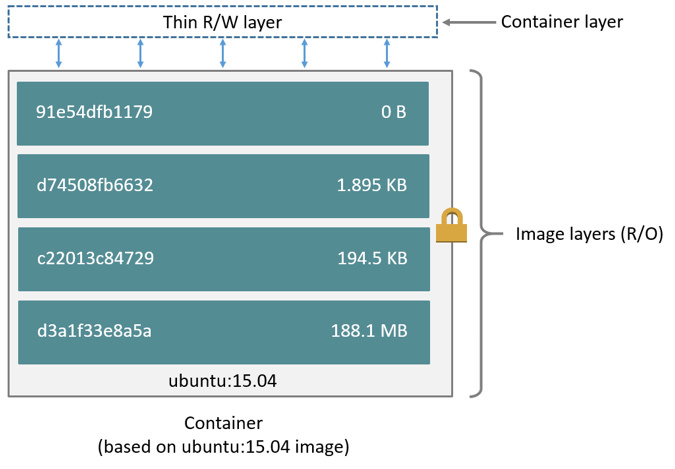
\includegraphics[width=1\textwidth]{relazione-tirocinio/Chapter-2/container-layers.jpg}
\end{figure}
Questo tipo di architettura favorisce la condivisione di risorse, infatti se ho più container creati partendo dalla stessa immagine, le modifiche verranno effettuate solo nell'ultimo livello dei rispettivi container condividendo tutti i livelli sottostanti\cite{aboutstoragedrivers}.
Dato che tutti i dati scritti dal container vengono salvati nell'ultimo livello modificabile, quando il container viene distrutto vengono persi anche i dati scritti dal container.
La persistenza dei dati può essere garantita da due metodi differenti.
Un \textbf{volume} è una parte del filesystem amministrata da Docker in cui solo i processi Docker possono avere accesso. Solitamente risiedono in \texttt{/var/lib/docker/volumes/}.
Un \textbf{bind mount} differisce dal volume in due punti: ogni processo può avere accesso ai dati e può risiedere ovunque nel sistema. 
Questo garantisce che se il container va in uno stato di errore o la macchina dove viene deployato il container si spegne, i dati vengono comunque salvati in un disco fisso.
\\
Differisce dalla \textbf{virtualizzazione} \cite{dockervsvm2} in:

\begin{itemize}
    \item Deployment semplificato: i container possono essere creati, distrutti e replicati in qualsiasi ambiente in modo semplice e veloce.
    \item Ampia portabilità: permette di impacchettare l'applicativo in un singolo elemento facilmente distribuibile.
    \item Prestazioni: Sono più leggeri e veloci delle macchine virtuali perché non richiedono una virtualizzazione del sistema operativo e condividono le risorse tra i vari container.
    \item Isolamento: Per quanto un container Docker isoli i vari applicativi, una Virtual Machine garantisce un maggiore isolamento.
\end{itemize}

\begin{figure}[ht]
\caption{Container vs Virtualizzazione}
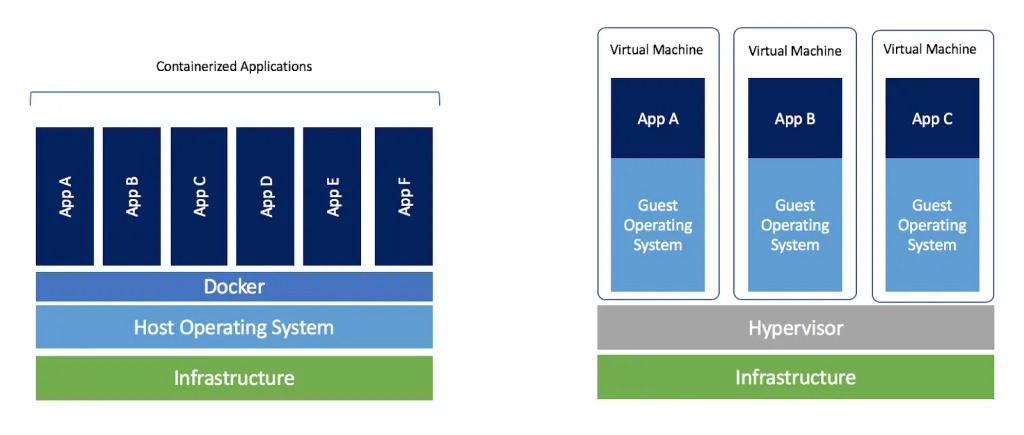
\includegraphics[width=1\textwidth]{relazione-tirocinio/Chapter-2/vm-c.jpg}
\end{figure}
Questa divisione netta fra i container e la condivisione delle risorse per aumentare le prestazioni si prestano molto al caso in esame. Ogni container avrà in esecuzione una instanza di node-red configurata con i dati di un determinato gruppo.
Come si può notare dai grafici nelle prossime pagine, tratti dallo studio di \textit{Potdar et al.}\cite{dockervsvm}, ci sono molti vantaggi prestazionali nell'utilizzo di container Docker invece di macchine virtuali.

\begin{figure}
    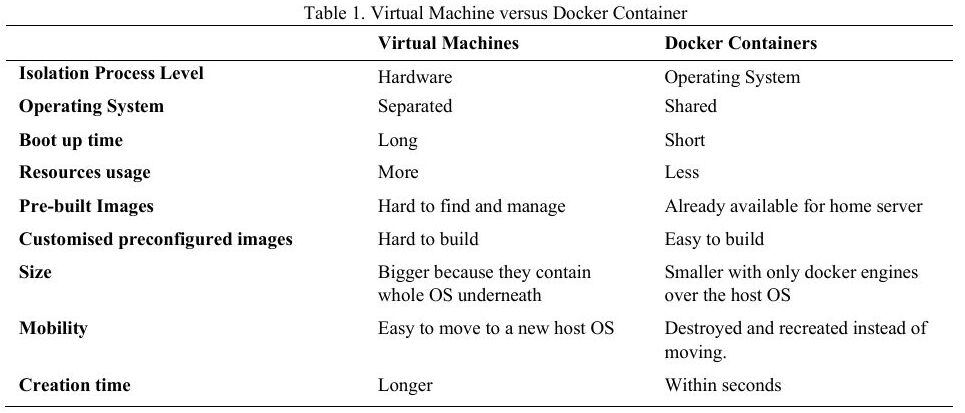
\includegraphics[width=1\textwidth]{relazione-tirocinio/Chapter-2/docker-vm-1.jpg}
    \label{fig:docker-vm-1}
\end{figure}
La comparazione nei test delle prestazioni della CPU è stato fatta utilizzando gli strumenti sysbench, Phoronix e Apache benchmark. È stato utilizzato il metodo del \textbf{massimo numero primo}.
Viene dato un tempo massimo, in questo caso 60 secondi e deve essere dato in risultato il numero primo massimo minore di 50000 con 4 thread operativi.
Per il test di compressione dati è stato utilizzato 7-Zip con un file di 10GB.
Le prestazioni della memoria RAM (utilizzando RAM speed/SMP) sono state misurate con gli strumenti INTmark e FLOATmark che misurano le prestazioni massime possibili di cache e memoria mentre leggono e scrivono blocchi individuali di dati.
In un ulteriore test è stato utilizzato un caso particolare, cioè Eigth Queen, una simulazione di un problema del gioco degli scacchi.
\begin{figure}
\begin{tabular}{cc}
  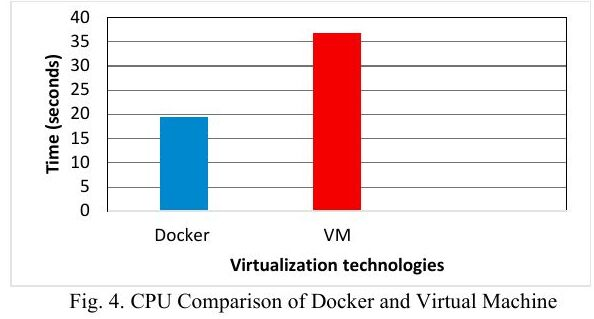
\includegraphics[width=0.5\textwidth]{relazione-tirocinio/Chapter-2/docker-vm-2.jpg} &   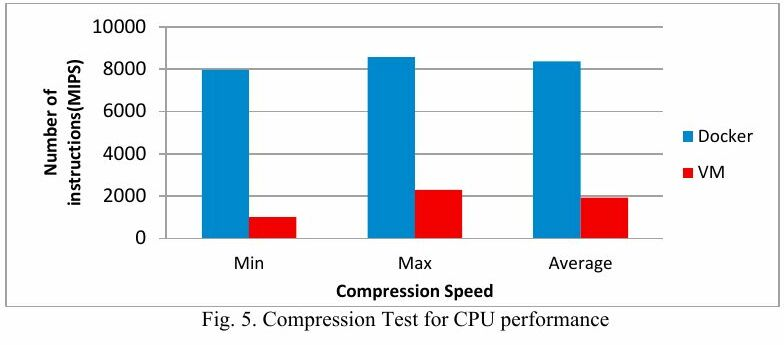
\includegraphics[width=0.5\textwidth]{relazione-tirocinio/Chapter-2/docker-vm-3.jpg} \\
 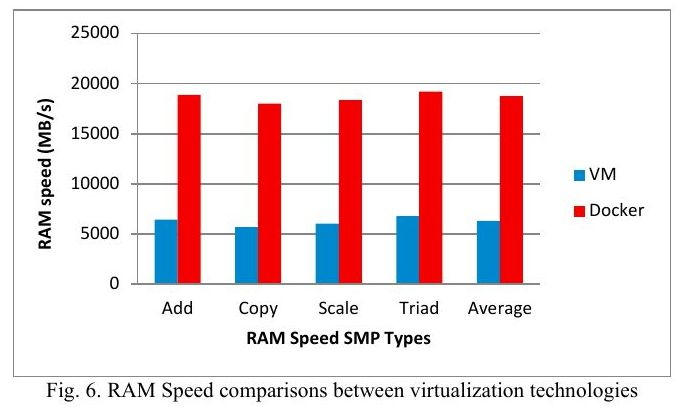
\includegraphics[width=0.5\textwidth]{relazione-tirocinio/Chapter-2/docker-vm-4.jpg} &   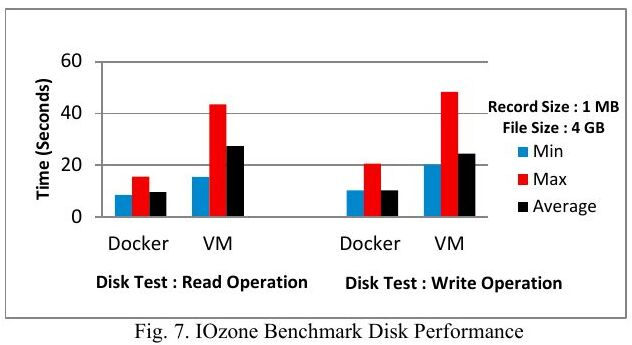
\includegraphics[width=0.5\textwidth]{relazione-tirocinio/Chapter-2/docker-vm-5.jpg} \\
 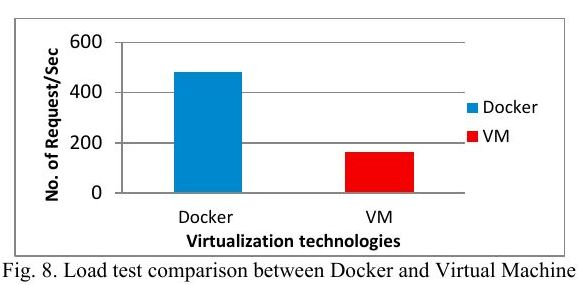
\includegraphics[width=0.5\textwidth]{relazione-tirocinio/Chapter-2/docker-vm-6.jpg} &   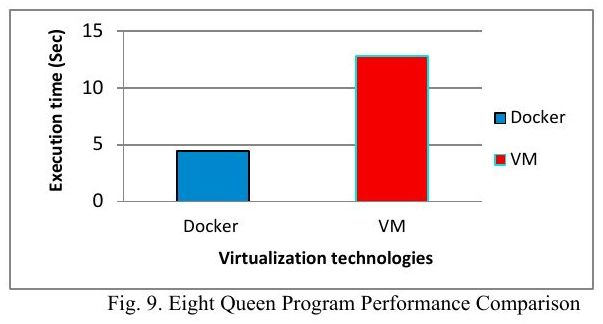
\includegraphics[width=0.5\textwidth]{relazione-tirocinio/Chapter-2/docker-vm-7.jpg} \\
\end{tabular}
\end{figure}
Come possiamo notare dai grafici, le prestazioni dei container Docker sono di gran lunga superiori rispetto alle macchine virtuali. Dato che l'immagine del nostro sistema è identica per tutti i container si ha un netto miglioramento delle performance utilizzando container perché tutti i container condividono la stessa immagine di base.

\vspace{0.02\textwidth}
\begin{center}
Esempio di immagine utilizzata in SeismoCloud partendo dalla immagine di Node-RED su DockerHub come base(\href{https://hub.docker.com/r/nodered/node-red/}{https://hub.docker.com/r/nodered/node-red/}).
\end{center}

\begin{lstlisting}[language=docker]
# from nodered/node-red:1.0.6-12
FROM nodered/node-red@sha256:82f367ab41d19e3ebd5e9b1cc62e4f615d4b4be4fa8bc83f1bf5441ba8c0d32a

# Qui vengono settate tutte le variabili d'ambiente
ENV VAR="hello-world"

# Vengono indicati i volumi per la persistenza dei dati
VOLUME /volume

# Tutte le cartelle vengono copiate nell'immagine
COPY data data

RUN chown -R node-red data
USER node-red

RUN npm install #Tutti i nodi custom necessari

CMD ["npm", "start"]
\end{lstlisting}
La seconda riga differisce dall'immagine definita nel Dockerfile di esempio per un codice dopo la definizione dell'immagine di partenza.
Questo codice è formato da due campi:\\ \texttt{algoritmo:valore-esadecimale}.
In questo caso l'algoritmo utilizzato è \texttt{sha256}. Viene calcolato lo stesso algoritmo su tutti i livelli che compongono l'immagine, successivamente viene creato un file \texttt{Manifest}, a cui poi viene calcolato lo stesso algoritmo di hash che corrisponde al digest dell'immagine. Ovviamente questo hash serve a verificare che effettivamente quello che è stato scaricato corrisponde all'immagine desiderata. Non utilizzando un hash, ma come scritto prima un tag (ubuntu:\texttt{18:04}) scarico una immagine ma non verifico il contenuto che appunto potrebbe essere manomesso. 

\vspace{0.02\textwidth}
Il deploy di tanti servizi può essere semplificato utilizzando \textbf{docker-compose}.
\begin{lstlisting}[language=docker-compose-2]
version: '3'
services:

  seismocloud-nodered-1:
    restart: always
    image: seismocloud-nodered:latest
    environment:
      - NUM_GROUP = 2222345435
    ports:
      - 1880:1880
    volumes:
      - ./volume:/volume
      
  seismocloud-nodered-2:
    restart: always
    image: seismocloud-nodered:latest
    environment:
      - NUM_GROUP = 2222345436
    ports:
      - 1880:1880
    volumes:
      - ./volume:/volume
\end{lstlisting}
Compose è uno strumento per definire ed eseguire applicazioni Docker multi-container. Si usa un file di tipo YAML per definire tutti i componenti ed impostare il servizio.
Vengono creati i file Dockerfile relativi a tutte le immagini che devono essere costruite ed un file \texttt{docker-compose.yml}.
In questo caso appunto, vengono eseguiti due servizi node-red con immagine customizzata (seismocloud-nodered) per due differenti gruppi.
Con un singolo comando si possono eseguire tutti i servizi configurati in precedenza (\textit{docker-compose up}), oppure stopparli (\textit{docker-compose stop}) e con un altro farli ripartire (\textit{docker-compose restart}).
Se, mentre tutti i servizi sono in esecuzione, si vuole modificare lo stato di uno solo è possibile farlo con i comandi di Docker.
\clearpage

Qui con \textbf{node-RED instance} si intende un container per un gruppo specifico.
Il container interagisce con l'interfaccia web per garantire l' autenticazione di un utente; interagisce con i sismometri attraverso i vari protocolli per lo scambio di dati (HyperText Transfer Protocol, Message Queue Telemetry Transport).
Interagisce con gli smartphone nel caso in cui gli utenti decidono di ricevere notifiche push o altri tipi di alert (messaggi Telegram o altra applicazione).
Con il data server scambia informazioni attraverso il broker mqtt e riceve informazioni sul gruppo (statistiche e dati dei sismometri) attraverso le API.
\begin{figure}[ht]
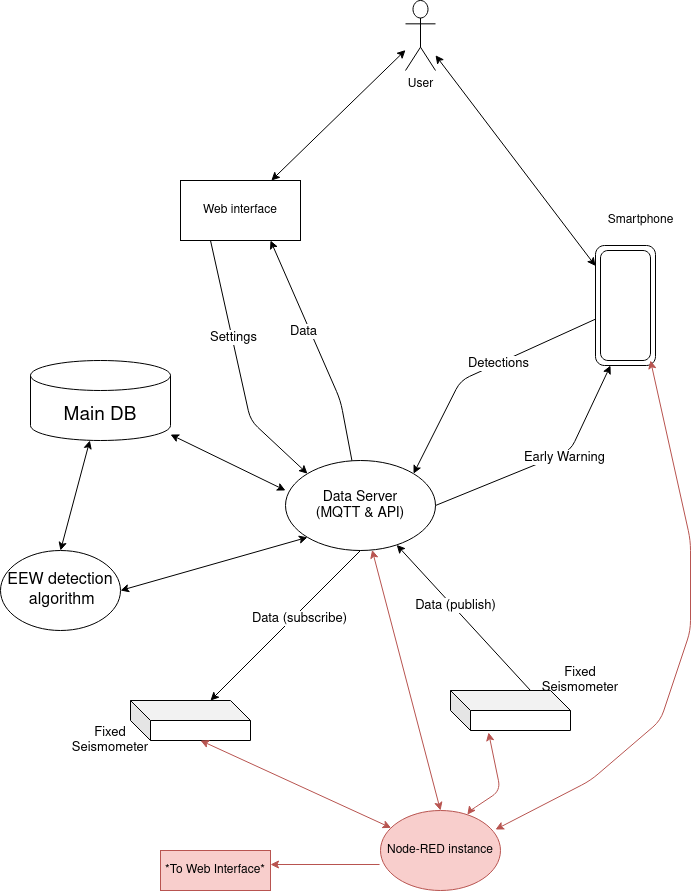
\includegraphics[width=0.9\textwidth]{relazione-tirocinio/Chapter-2/architettura-seismocloud2.png}
\end{figure}

% ======================================= CHAPTER 3 ================================================
\chapter{Implementazione delle funzionalità}

\section{Sistema Legacy}

Come è stato accennato nella descrizione dell'architettura del sistema SeismoCloud (Cap 1.3), è presente un sistema di End User Development. In particolare è possibile programmare della azioni quando si verificano determinate condizioni pur non avendo competenze in programmazione software.
Le condizioni disponibili sono tre: quando $n$ (o un solo) sismometri vibrano/sono accesi, quando un sismometro entra in una scuola, oppure la notifica di un Earthquake Early Warning.
Le possibilità per il metodo di notifica sono quattro: un messaggio tramite Telegram, una notifica push ai membri del gruppo, un widget e la pubblicazione di una API.
\begin{figure}[ht]
\label{legacy1}
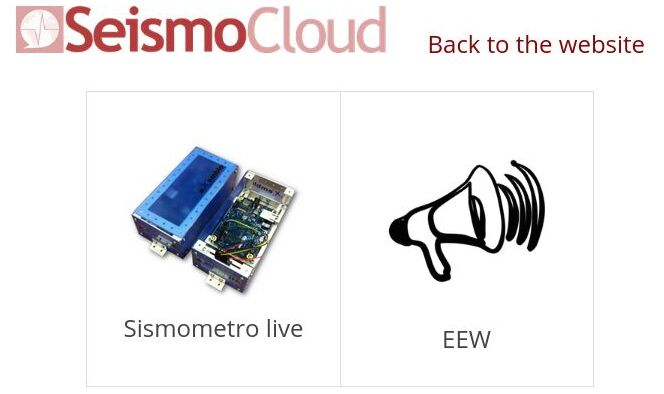
\includegraphics[width=1\textwidth]{relazione-tirocinio/Chapter-3/eud-legacy-1.jpg}
\end{figure}
Visto che i dati prodotti sono tanti, sarebbe molto utile ampliare il range di condizioni ad un più vasto campo, tenendo in conto anche di tutti i dati che non vengono considerati in questo sistema, ma che vengono comunque collezionati dai sismometri (temperatura, indirizzi IP, soglia di Quake, rssi, reboot..).
Sarebbe ancora più utile lasciare completa \textbf{libertà all'utente} (sotto alcune restrizioni di sicurezza) integrando il sismometro con l'ambiente locale potenziando così le funzionalità e l'utilità di un sismometro.
Quindi, un primo problema del sistema legacy di EUD è sicuramente la rigidità nelle azioni messe a disposizione per l'utente.
Con Node-RED, possono essere costruite tantissime azioni automatizzate dato l'elevato numero di funzionalità offerte.
Si potrebbe quindi decidere di riavviare un sismometro ogni volta che la temperatura supera i 50$^{\circ}$C. Oppure mandare una mail, pubblicare un tweet e scaricare un file quando vengono rilevate tre vibrazioni nello stesso minuto.
Un ulteriore vantaggio è l'integrazione con i dispositivi smart/IoT. Node-RED è stato ideato e viene mantenuto come strumento per la programmazione flow-based per ambienti IoT/industriali. Ad esempio se si possiede qualche dispositivo per una smart home (telecamere, smart TV, frigorifero etc...) possono essere collegati al sismometro ed automatizzati basandosi anche su eventi sismici.
Il tutto non deve risultare complesso, deve essere possibile l'utilizzo per utenti non esperti in informatica o elettronica, ma allo stesso tempo i più competenti devono poter sfruttare le loro abilità.
La soluzione a questo bisogno dovrebbe essere: \textit{facilmente utilizzabile, sicura, affidabile e performante}.
Senza ombra di dubbio un punto di forza del precedente sistema è l'elevata \textbf{usabilità}. Infatti, essendo disponibili poche funzionalità e quindi pochi pulsanti è molto facile da comprendere.
Questa facilità d'uso deve essere mantenuta anche nel nuovo sistema per non escludere utenti non tecnicamente competenti.
Il vecchio sistema di EUD rende possibile, come già introdotto, la programmazione di azioni condivisa con il proprio gruppo di appartenenza.
Questa impostazione viene ripresa nel nuovo sistema, quindi ogni membro di un gruppo deve poter accedere alla propria \textit{istanza di gruppo di Node-RED} per programmare le azioni desiderate con tutti e soli i sismometri appartenenti al gruppo. Le azioni si possono basare su dati provenienti da tutta la rete.
La ragione principale di questa scelta è che in questo modo si hanno molti più dati disponibili.

\begin{figure}[ht]
\label{legacy2}
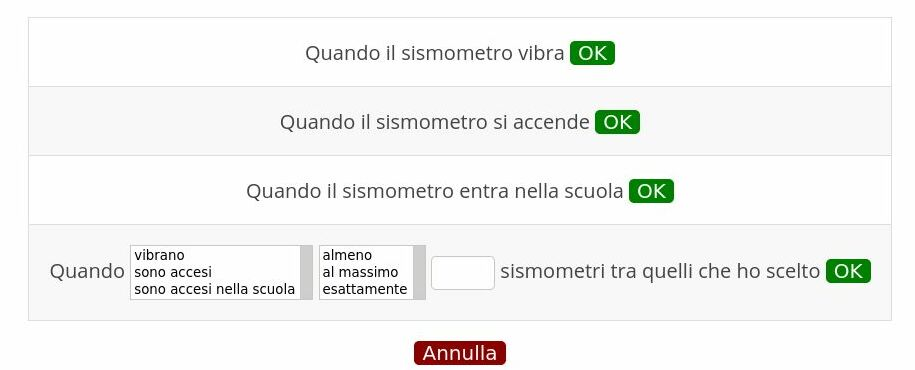
\includegraphics[width=1\textwidth]{relazione-tirocinio/Chapter-3/eud-legacy-2.jpg}
\end{figure}
\clearpage

\section{Difficoltà e limiti nell'uso di Node-RED}

L'immagine di partenza di Node-RED fornisce alcune funzionalità di base. Nella palette di sinistra sono presenti sei sezioni (common, function, network, sequence, parser, storage) che raggruppano i vari nodi in base all'argomento di appartenenza. È stato già anticipato che questo strumento viene utilizzato nell'industria e ha un grande potenziale, possono essere programmate un vasto range di azioni utilizzando molte tecnologie e protocolli differenti. Sono presenti anche azioni che non possono essere programmate ad \textit{alto livello}, cioè si deve scendere nei tecnicismi della tecnologia utilizzata. Un esempio di ciò è l'\textbf{invio di una richiesta di sottoscrizione ad un topic verso il broker mqtt di SeismoCloud}. 

\begin{figure}[hbt]
    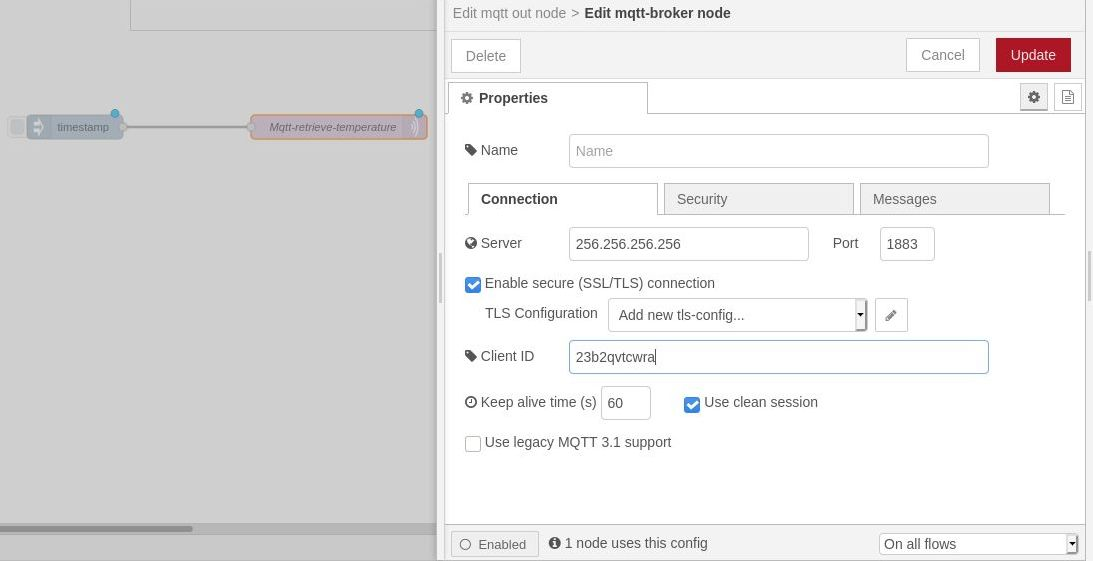
\includegraphics[width=1\textwidth]{relazione-tirocinio/Chapter-3/mqtt-legacy-1.jpg}
    \label{fig:mqtt-legacy-1}
\end{figure}

Il problema che si nota qui è l'elevato numero di impostazioni e settaggi che l'utente deve inserire per configurare correttamente un client MQTT per ricevere un solo tipo di dato.
Vengono richieste competenze in questa specifica tecnologia e non solo (anche nozioni generali di reti). Ad esempio, si deve inserire l'indirizzo IP del server (in questo caso scelto appositamente non esistente come esempio) \texttt{256.256.256.256}, la porta di riferimento \texttt{1883}, un client ID ed un keep alive time. Se si vuole anche configurare una connessione sicura tramite \textit{SSL/TSL} devono essere configurati anche i relativi parametri per la cifratura dei dati.
Se il server è protetto da username e password (come nel caso SeismoCloud), c'è un tab anche per quello. Quindi qui c'è anche un problema di sicurezza: per fornire dati agli utenti devo fornire loro anche le informazioni di autenticazione ed accesso al server.
Inoltre, ovviamente, l'utente deve essere a conoscenza di come sono formati tutti i topic di cui ha bisogno.
Se inoltre si vogliono pubblicare messaggi e non solamente riceverli si hanno a disposizione più tipologie di messaggi per comunicare con il server.
Il protocollo MQTT inoltre ha il particolare \textit{Quality of Service} che funziona in questo modo:
Si può settare un valore numerico (0 , 1 o 2) che corrisponde al grado di accuratezza ed affidabilità nella consegna dei messaggi.

\begin{itemize}
    \item QoS 0: Con questa impostazione si ha un servizio \textit{orientato alle prestazioni con il minor impiego di energia}. Il client non riceve feedback dell'avvenuta consegna del messaggio.
    \item QoS 1: Quando si riceve  un messaggio con QoS uguale ad 1, si deve inviare un messaggio di acknowledgment che certifica che la ricezione è correttamente avvenuta. Specularmente, se si invia un messaggio con QoS 1 allora devo aspettare il feedback. Nel caso di un problema di rete (ad esempio congestione) e il mittente non riceve in un determinato lasso di tempo l'acknowledgment rinvierà di nuovo il messaggio. \textit{Questo può portare ad avere messaggi duplicati}.
    \item QoS 2: È la modalità più costosa in termini di sforzo (in modo relativo, il protocollo è progettato per una buona gestione delle risorse). Vengono inviati più messaggi per confermare la ricezione ed evitare eventuali duplicati.
\end{itemize}
Ovviamente non esiste un valore QoS migliore in assoluto, ma dipende dal messaggio e dallo scopo di esso.
Inoltre questo fa comprendere quante competenze sono richieste per l'invio di un messaggio con protocollo MQTT.
Ne esistono differenti di protocolli disponibili, quindi la conoscenza tecnica richiesta è elevata pur non richiedendo esperienza in programmazione attraversi dei linguaggi.

\begin{figure}[hbt]
    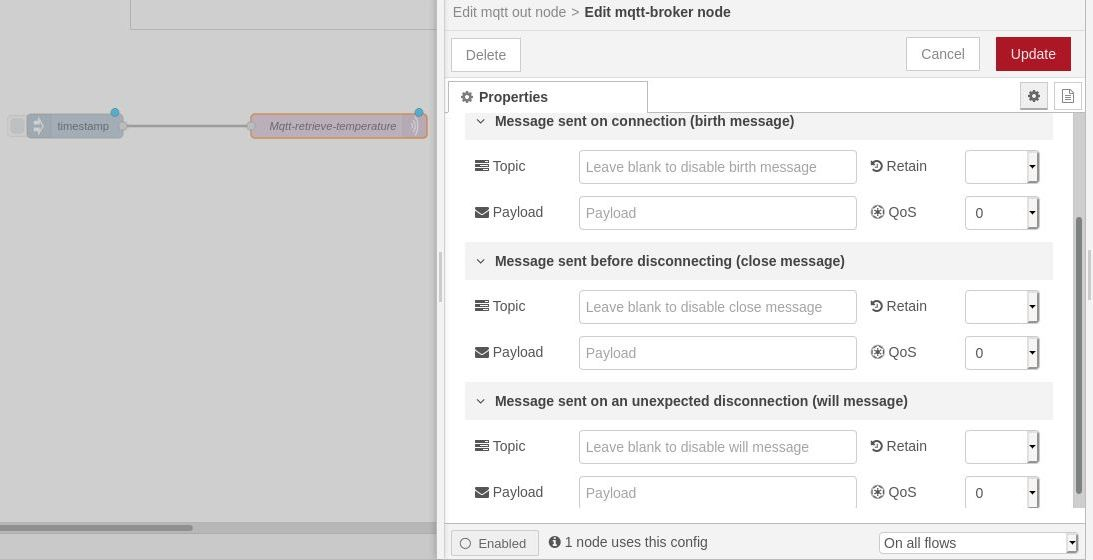
\includegraphics[width=1\textwidth]{relazione-tirocinio/Chapter-3/mqtt-legacy-2.jpg}
    \label{fig:mqtt-legacy-2}
\end{figure}

Quindi bisogna semplificare tutto questo processo minimizzando il numero di interazioni con l'utente e dando per scontati tutti i dati che sono già noti al sistema SeismoCloud.
Questo servirà a semplificare e rendere più usabile il sistema, considerando che il sistema precedente nascondeva tutte queste configurazioni aggiuntive.

\clearpage

\section{Implementazione delle funzionalità tramite nodi}

Come è stato introdotto, tutte le funzionalità aggiuntive personalizzabili sono implementate tramite \textit{nodi}.
\textbf{L'obiettivo principale è cercare di costruire nodi che hanno la minima configurazione necessaria con il massimo delle funzionalità offerte}. 

\subsection{Come è costruito un nodo}

I nodi sono moduli NPM ed hanno bisogno di un file Javascript per le funzionalità programmate, un file HTML per il layout ed un file JSON (chiamato \textit{package.json}) per pacchettizzarlo in un modulo.
Il file package.json può essere prodotto in modo automatico con il comando fornito dal package manager \texttt{npm init}.
\begin{lstlisting}[language=Javascript]
{
    "name" : "node-red-contrib-example-lower-case",
    ...
    "node-red" : {
        "nodes": {
            "lower-case": "lower-case.js"
        }
    }
}
\end{lstlisting}

\begin{lstlisting}[language=Javascript]
module.exports = function(RED) {
    function LowerCaseNode(config) {
        RED.nodes.createNode(this,config);
        var node = this;
        node.on('input', function(msg) {
            msg.payload = msg.payload.toLowerCase();
            node.send(msg);
        });
    }
    RED.nodes.registerType("lower-case",LowerCaseNode);
}
\end{lstlisting}
Qui abbiamo un esempio di file Javascript. Nella riga \texttt{1} il modulo esporta una funzione che viene eseguita quando il runtime Node-RED viene eseguito. La funzione definisce un solo input \texttt{RED}, il quale è un oggetto che garantisce l'accesso alle API del runtime RED.
Dalla riga \texttt{2} in poi abbiamo la definizione del nodo, viene creato un nuovo nodo con le configurazioni di base (riga \texttt{3}). Dalla riga \texttt{5} alla riga \texttt{8} viene definito il comportamento quando il nodo riceve un input, ossia viene ricevuto l'oggetto \texttt{msg}, viene estratto il \texttt{msg.payload} e viene trasformato in minuscolo.
Successivamente viene restituito in output l'oggetto \texttt{msg}.
Nella riga \texttt{10} viene poi aggiunta al runtime api la funzione appena sopra definita tramite il nome ``lower-case".

\begin{lstlisting}[language=Javascript]
<script type="text/javascript">
    RED.nodes.registerType('lower-case',{
        category: 'function',
        color: '#a6bbcf',
        defaults: {
            name: {value:"lower-case"}
        },
        inputs:1,
        outputs:1,
        icon: "file.png",
        label: function() {
            return this.name||"lower-case";
        }
    });
</script>

<script type="text/html" data-template-name="lower-case">
    <div class="form-row">
        <label for="node-input-name"><i class="fa fa-tag"></i> Name</label>
        <input type="text" id="node-input-name" placeholder="Name">
    </div>
</script>

<script type="text/html" data-help-name="lower-case">
    <p>A simple node that converts the message payloads into all lower-case characters</p>
</script>
\end{lstlisting}
Infine abbiamo il file HTML che definisce il layout del nodo.
Nella riga \texttt{2} viene associata tutta la definizione delle impostazioi che segue con il nodo chiamato ``lower-case".
Viene associata una categoria al nodo alla riga \texttt{3}. La categoria è uno strumento utile per l'usabilità, infatti permette di raggruppare nodi simili sotto lo stesso insieme. In questo caso viene inserito all'interno di \textit{function} essendo una funzione Javascript che riceve e modifica l'input.
Viene poi assegnato un colore al nodo in dicitura esadecimale uguale per tutti i nodi della stessa categoria, dei parametri di default (in questo caso solamente il nome del nodo), il numero di input e output accettati, un file PNG per associare al nodo un logo che ricorda l'azione che la funzione svolge.

\begin{figure}[ht]
    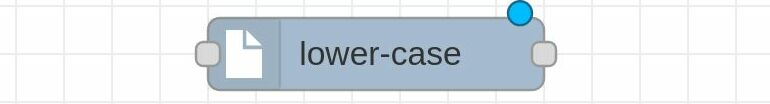
\includegraphics[width=1\textwidth]{relazione-tirocinio/Chapter-3/lower-case-1.jpg}
    \label{fig:lower-case-1}
\end{figure}

\begin{figure}[ht]
    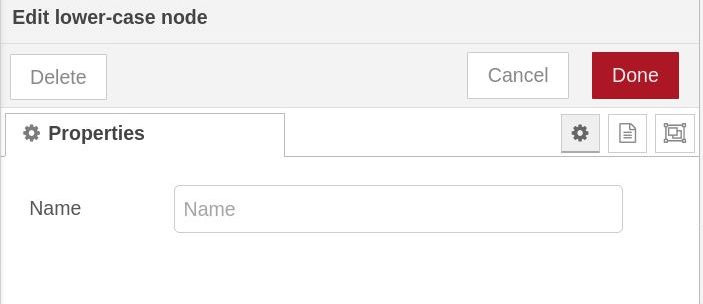
\includegraphics[width=1\textwidth]{relazione-tirocinio/Chapter-3/lower-case-2.jpg}
    \label{fig:lower-case-2}
\end{figure}

\subsection{Configurazione Node-RED}

Quando Node-RED viene eseguito deve essere presente il file \texttt{settings.js} dove vengono settate tutte le configurazioni\cite{noderedconfig}.
Sono disponibili cinque sezioni di configurazione: configurazione del runtime, dell'editor e dei suoi temi, della dashboard e dei nodi.
Questo file offre molte possibilità di configurazione, ma qui vengono esposte solo quelle utilizzate nel sistema EUD di SeismoCloud.
Come è stato spiegato nel paragrafo 2.2, i flussi creati vengono salvati tramite un file JSON che può essere settato tramite il valore \texttt{flowFile: $<$flowsfilename$>$.json}.
I nodi vengono cercati dal runtime all'interno della cartella definita da \texttt{nodesDir} (default \texttt{\$HOME/.node-red/nodes}).
È possibile definire una porta dedicata al servizio, di default è 1880.
Sono disponibili vari livelli di logging:
\begin{itemize}
    \item fatal: Solo gli errori che rendono l'applicativo inutilizzabile sono registrati
    \item error: Registra gli errori che sono ritenuti fatali per una particolare richiesta + fatal errors
    \item warn: Registra problemi che non sono fatali + errors + fatal errors
    \item info: Registra informazioni riguardo l'esecuzione generale dell'applicativo + warn + error + fatal errors
    \item debug: Registra informazioni più verbose rispetto ad info + info + warn + error + fatal errors
    \item trace: Registra log dettagliati + debug + info + warn + error + fatal errors
\end{itemize}

Come si può facilmente notare \texttt{fatal} corrisponde al meno verboso e gradualmente si aumenta fino ad arrivare a loggare ogni singola informazione. Di default il livello è settato ad \texttt{info}; viene lasciato quest'ultimo perché essendo un sistema appena creato e non maturo è fondamentale una attività intensa dei log, utili a fornire feedback e segnalare eventuali errori; non viene utilizzato il \texttt{debug} perché troppo verboso e non adatto.

Per quanto riguarda la configurazione dell'editor, qui si ha la possibilità di settare le categorie per i nodi. Di default sono presenti: \texttt{['subflows', 'common', 'function', 'network', 'sequence', 'parser', 'storage']}; nel sistema invece sono state rimosse le categorie \texttt{storage} e \texttt{network} (nel capitolo 4 vengono analizzate in dettaglio le motivazioni) e sono state aggiunte le categorie \texttt{SeismometerData} e \texttt{apiSeismocloud}.
I nodi che rientrano nelle categorie \texttt{network} e \texttt{storage} sono eliminati con questo comando:
\begin{lstlisting}
//EXCLUDING NODES FROM PALETTE:
  nodesExcludes: ['32-udp.js', '31-tcpin.js', '22-websocket.js', '21-httprequest.js', '21-httpin.js',
    '10-mqtt.js', '06-httpproxy.js', '05-tls.js', '90-exec.js', 'node-red-node-tail', '10-file.js',
    '23-watch.js'],
\end{lstlisting}

Queste sono le configurazioni disponibili per il tema dell'editor, utili soprattutto per una alta comprensibilità dell'interfaccia.
\begin{lstlisting}[language=Javascript]
editorTheme: {
    page: {
        title: "SeismoCloud EUD",
        favicon: "/absolute/path/to/theme/icon",
        css: "/absolute/path/to/custom/css/file",
        scripts: [ "/absolute/path/to/custom/script/file", "/another/script/file"]
    },
    header: {
        title: "SeismoCloud EUD",
        image: "/absolute/path/to/header/image", // or null to remove image
        url: "https://www.seismocloud.com/" // optional url to make the header text/image a link to this url
    },
    deployButton: {
        type:"simple",
        label:"Save",
        icon: "/absolute/path/to/deploy/button/image" // or null to remove image
    },
    menu: { // Hide unwanted menu items by id. see packages/node_modules/@node-red/editor-client/src/js/red.js:loadEditor for complete list
        "menu-item-import-library": false,
        "menu-item-export-library": false,
        "menu-item-keyboard-shortcuts": false,
        //"menu-item-help": {
            //label: "Alternative Help Link Text",
            //url: "http://example.com"
        //}
    },
    userMenu: false, // Hide the user-menu even if adminAuth is enabled
    palette: {
        editable: false, // Enable/disable the Palette Manager
        //theme: [ // Override node colours - rules test against category/type by RegExp.
        //    { category: ".*", type: ".*", color: "#f0f" }
        //]
    },
    projects: {
        enabled: false // Enable the projects feature
    }
},
\end{lstlisting}
È possibile aggiungere un titolo personalizzato alla pagina Web, una icona, del codice css e degli script personalizzati.
Nell'interfaccia c'è un header che ospita una immagine che può funzionare da link, nel nostro caso rimanda al sito SeismoCloud.
In alto a destra nell'interfaccia, il tasto Deploy (che appunto effettua il deploy dell'applicativo) è rinominato in \texttt{Save} perché più comprensibile ad un pubblico non esperto.
Nel menu è possibile far comparire o non comparire alcune funzionalità, nel caso SeismoCloud sono utili e perciò sono lasciate attive (ad esempio la possibilità di esportare ed importare flussi pronti tramite il file in formato json. Vari gruppi possono condividere un flusso complesso cambiando pochi dettagli). 
È stato disabilitato il palette manager perché consentiva di aggiungere nodi esterni alla palette tramite Internet, potenzialmente un problema di sicurezza (analizzato nel capitolo 4).
Anche la funzionalità projects per ora è disabilitata perché non necessaria, almeno per le prime release del sistema (Projects permette di avere un supporto per \texttt{Version Control System} come GitHub etc..).

Queste sono invece le impostazioni di configurazione dei nodi:
in millisecondi sono definiti i tempi di riconnessione e timeout per i vari protocolli e relative richieste.
\begin{lstlisting}[language=Javascript]
  // Retry time in milliseconds for MQTT connections
  mqttReconnectTime: 15000,

  // Retry time in milliseconds for Serial port connections
  serialReconnectTime: 15000,

  // Retry time in milliseconds for TCP socket connections
  socketReconnectTime: 10000,

  // Timeout in milliseconds for TCP server socket connections
  //  defaults to no timeout
  socketTimeout: 10000,

  // Maximum number of messages to wait in queue while attempting to connect to TCP socket
  //  defaults to 1000
  tcpMsgQueueSize: 1000,

  // Timeout in milliseconds for HTTP request connections
  //  defaults to 120 seconds
  httpRequestTimeout: 10000,

  // The maximum length, in characters, of any message sent to the debug sidebar tab
  debugMaxLength: 1000,
\end{lstlisting}

\subsection{Implementazione di nodi che utilizzano MQTT per i dati relativi ai sismometri}

Spiegazione nodi MQTT, codice e semplificazione rispetto a prima (immagini).

Come spiegato nel paragrafo 3.2 (Difficoltà e limiti nell'uso di Node-RED), un utente che non ha competenze tecniche informatiche potrebbe avere grandi difficoltà nel configurare un'azione piuttosto semplice.
L'obiettivo del lavoro svolto è di semplificare il più possibile la creazione di flussi Node-RED riducendo al minimo le competenze richieste e la configurazione da parte dell'utente.
Molti valori che vengono inseriti (e poi ripetuti nel caso di più nodi che utilizzano il protocollo MQTT) sono già a conoscenza del sistema SeismoCloud, perciò si è optato per la creazione di nodi customizzati che hanno già all'interno tutte le informazioni note.

Qui è presente la lista dei vari nodi creati per il sistema EUD di SeismoCloud; sono tutti moduli NPM che rispettano la definizione di modulo definita precedentemente in questo paragrafo.

\begin{itemize}
    \item node-red-contrib-rssi (Input: 0, Output: 1): Questo nodo produce in output l'indicatore di potenza del segnale ricevuto (RSSI), una misura stimata di quanto bene un dispositivo può ricevere segnali dal punto di accesso a cui è collegato.
    \item node-red-contrib-bssid (Input: 0, Output: 1): Questo nodo produce in output il BSSID, che identifica l'insieme di servizi di base del dispositivo. Il più delle volte è associato all'indirizzo MAC del punto di accesso a cui è collegato.
    \item node-red-contrib-essid (Input: 0, Output: 1): Questo nodo restituisce il nome del punto di accesso alla rete a cui è collegato il dispositivo.
    \item node-red-contrib-localip (Input: 0, Output: 1): Questo nodo restituisce l'indirizzo Ip nella rete locale del dispositivo.
    \item node-red-contrib-publicip (Input: 0, Output: 1): Questo nodo produce in output l'indirizzo Ip pubblico su Internet del dispositivo.
    \item node-red-contrib-threshold (Input: 0, Output: 1): Questo nodo restituisce la soglia utile al calcolo di un Earthquake Early Warning.
    \item node-red-contrib-alive (Input: 0, Output: 1): Questo nodo segnala che il dispositivo è attivo al momento. 
    \item node-red-contrib-timesync (Input: 0, Output: 1): Questo nodo sincronizza il timer del dispositivo.
    \item node-red-contrib-timereq (Input: 0, Output: 1): Questo nodo aiuta il precedente nella sincronizzazione.
    \item node-red-contrib-quake (Input: 0, Output: 1): Questo nodo produce in output i valori di una vibrazione del dispositivo. 
    \item node-red-contrib-disconnect (Input: 0, Output: 1): Questo nodo restituisce il segnale inviato quando un dispositivo viene disconnesso.
    \item node-red-contrib-reboot (Input: 1, Output: 1): Questo nodo segnala il riavvio del dispositivo. 
    \item node-red-contrib-temperature (Input: 0, Output: 1): Questo nodo restituisce il valore che indica la temperatura del dispositivo in $^{\circ}$C.
    \item node-red-contrib-probespeed (Input: 0, Output: 1): Questo nodo setta la velocità della sonda in Hz
    \item node-red-contrib-sigma (Input: 0, Output: 1): Questo nodo restituisce il valore \texttt{sigma} (utile al rilevamento di possibili scosse)
\item node-red-contrib-stream (Input: 0, Output: 1): Questo nodo restituisce (\texttt{on} / \texttt{off}) l'impostazione di ricezione dati dal server
    \item node-red-contrib-streamdata (Input: 0, Output: 1): ?
\end{itemize}

Tutti questi dati vengono inviati e ricevuti tramite il protocollo MQTT dal server e dal client. La maggior parte delle informazioni di configurazione non cambia, quindi sono stati creati per la maggiore parte di essi (tranne reboot e alive, spiegata in seguito la motivazione) nodi che funzionano allo stesso modo.
Dato che Node-RED utilizza NodeJS come runtime, il linguaggio utilizzato è Javascript e la libreria che aggiunge funzionalità riguardanti MQTT è \textbf{MQTT.js}.
La scelta è motivata dal codice open-source, dalla attiva community di utenti e sviluppatori e dalla maturità del progetto \cite{mqttjs}.
Per la seguente spiegazione viene preso come esempio \textbf{node-red-contrib-rssi}.
Il nucleo delle funzionalità è all'interno del file Javadcript, in questo caso \texttt{rssi.js}.
Dalla riga 1 alla riga 5 viene creato il nodo con le configurazioni di base (config) e vengono istanziate alcune variabili per facilità di lettura.
\begin{lstlisting}[language=Javascript]
module.exports = function (RED) {
  function RssiNode(config) {
    RED.nodes.createNode(this, config);
    var node = this;
    var seismometer = config.seismometer
\end{lstlisting}
\clearpage
Qui dalla riga 39 alla 52 viene creato effettivamente il client MQTT e settato il topic. In questo caso il valore \texttt{seismometer} è il codice identificativo del sismometro.
Viene poi creata una funzione callback in risposta ad un evento di connessione: quando il client MQTT si connette si deve iscrivere al topic selezionato, se il tutto va a buon fine viene loggata l'informazione, altrimenti stampato l'errore.
\begin{lstlisting}[language=Javascript, firstnumber=39]
    //===== Connect the client to the server and  define the topic =====
    var client = mqtt.connect(mqtt.IClientOptions);
    var topic = 'sensor/' + seismometer + '/rssi';
    
    //====== on connect event, subscribe to the topic =====
    client.on('connect', function () {
        client.subscribe(topic, function (err) {
            if (!err) {
          node.log("Client succesfully subscribed to " + topic + " !");
        } else {
          console.log(err)
        }
      })
    });
\end{lstlisting}
Dalla riga 60 in poi vengono definite tutte le altre funzioni callback per gli altri eventi: quando viene ricevuto un messaggio, quando avviene un errore di connessione dati MQTT o un errore della configurazione del nodi e quando il nodo viene distrutto dall'utente. Infine viene aggiunto alle API runtime di Node-RED il nodo \texttt{RssiNode} con il nome di \textit{rssi}.
\begin{lstlisting}[language=Javascript,firstnumber=60]
        //===== on message event, log on console and send msg =====
        client.on('message', function (topic, message) {
          node.log("Message received from " + topic + ":" + message.toString());
          var msg = { payload: message.toString() };
          node.send(msg);
        });

        //======= on error event, log on console ========
        client.stream.on('error', function () {
          node.log("MQTT ERROR on " + topic);
        });

        //== on error event, log error on console and display error status ==
        node.on("error", function (err) {
          node.status({ fill: "red", shape: "ring", text: "node-red:common.status.error" });
          node.error(err.toString());
        });

        //======== on close event, log on console and destroy client ========
        node.on('close', function () {
          client.end()
          node.log("Client succesfully unsubscribed by " + topic + " !");
        });
      });
    });
  }
  RED.nodes.registerType("rssi", RssiNode);
}
\end{lstlisting}
\clearpage

Il codice mostrato sopra definisce le funzionalità del nodo, per impostare il layout abbiamo bisogno di un file HTML, in questo caso \textbf{rssi.html}.
In questo snippet di codice viene definito il menù a tendina che permette di scegliere tra i vari sismometri del gruppo il sismometro selezionato.
\begin{lstlisting}[language=Javascript,firstnumber=45]
<script type="text/html" data-template-name="rssi">
    <div class="form-row">
        <label for="node-input-name"><i class="icon-tag"></i> Name</label>
          <input type="text" id="node-input-name" placeholder="Name">
    </div>
    <div class="form-row">
    <label for="node-input-seismometer"><i class="icon-tag"></i> Seismometer</label>
        <select id="node-input-seismometer">
        </select>
    </div>
</script>
\end{lstlisting}

\begin{figure}[ht]
    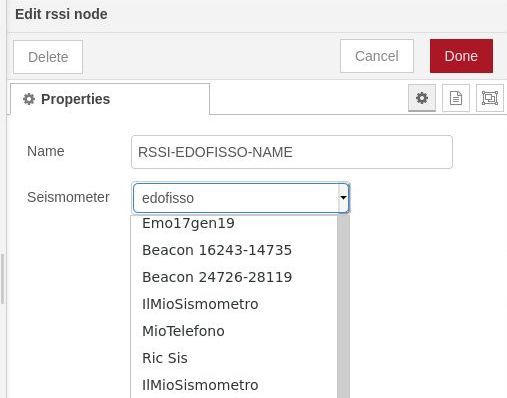
\includegraphics[width=1\textwidth]{relazione-tirocinio/Chapter-3/menu.jpg}
    \caption{Dati necessari per la configurazione di un nodo SeismoCloud}
    \label{fig:menu}
\end{figure}

\clearpage

Tramite il file \texttt{package.json} invece vengono definite impostazioni di base per il modulo.
\begin{lstlisting}
{
  "name": "red-contrib-rssi",
  "version": "1.0.0",
  "description": "This node returns periodically information about Received signal strength indication. INPUT: 0 | OUTPUT: 1 (string)",
  "main": "rssi.js",
  "scripts": {
    "test": "echo \"Error: no test specified\" && exit 1"
  },
  "dependencies": {
    "mqtt": "3.0.0",
    "url-parse": "1.4.7"
  },
  "node-red": {
    "nodes": {
      "rssi": "rssi.js"
    }
  },
  "author": "edoardottt",
  "license": "ISC"
}
\end{lstlisting}

\begin{figure}[ht]
    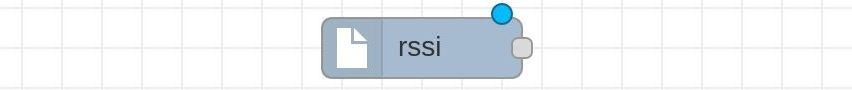
\includegraphics[width=1\textwidth]{relazione-tirocinio/Chapter-3/rssi-1.jpg}
    \label{fig:rssi-1}
\end{figure}
\begin{figure}[ht]
    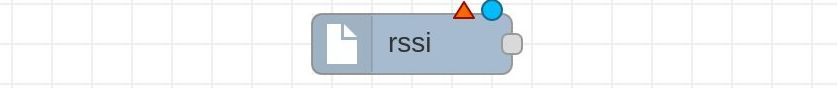
\includegraphics[width=1\textwidth]{relazione-tirocinio/Chapter-3/rssi-2.jpg}
    \label{fig:rssi-2}
\end{figure}
Le figure mostrate qui sopra raffigurano due nodi rssi inseriti nel workspace.
Entrambi hanno un cerchio azzurro in alto a destra, mentre solo secondo ha anche un triangolo arancione.
Il cerchio blu sta ad indicare che ancora non sono state salavate le modifiche effettuate al flusso, mentre il triangolo arancione indica la non corretta (o mancante) configurazione del nodo.
Per configurare il nodo bisogna definire il sismometro a cui il nodo si riferisce, è necessario un doppio click sinistro sul nodo, comparirà il menu laterale (figura \ref{fig:menu}) che consente di selezionare uno tra i dispositivi nel gruppo.
Il cerchio blu è inserito di default nell'interfaccia da Node-RED, l'altro segnale è stato aggiunto successivamente per aiutare l'utente nel processo di creazione dei flussi.

I nodi che hanno un compito speciale sono \textbf{Alive} e \textbf{Reboot}.
Il nodo Alive quando viene caricato dal runtime esegue una chiamata alle API di SeismoCloud per ottenere tutti i dati dei sismometri che sono registrati nel gruppo selezionato. Quest'ultimi (nome del dispositivo, identificativo alfanumerico, latitudine e longitudine, timestamp di ultima attività, tipo e versione) verranno poi messi a disposizione ed utilizzati dagli altri nodi e dal runtime stesso per eseguire dei controlli e per settare tutte le informazioni che non devono essere inserite dall'utente proprio perché il sistema ne è già a conoscenza.
Il nodo reboot invece quando riceve in input qualcosa (non ci sono controlli, può essere una stringa, un numero, in generale un valore qualsiasi) pubblica un messaggio (in questo caso un semplice ''y") sul topic dedicato al sismometro selezionato per effettuare il riavvio dello stesso.
\begin{lstlisting}[language=Javascript, firstnumber=80]
    //== on input event, publish a message on this topic ==
    node.on('input', function (msg) {
        var message = "y"
        client.publish(topic, message, function (err) {
            if (!err) {
            node.log("Client succesfully published to " + topic + " !");
            var msg = { payload: "reboot" };
            node.send(msg);
          }
        })
    });
\end{lstlisting}

\subsection{Implementazione di nodi che utilizzano API SeismoCloud per statistiche e informazioni sul sistema}

Spiegazione nodi API, codice, funzionalità offerte e semplificazione rispetto a prima (immagini).

\begin{itemize}
    \item node-red-contrib-get-seismometer-info (Input: 1, Output: 1): Questo nodo quando riceve un input restituisce le informazioni del dispositivo selezionato.
    \item node-red-contrib-list-earthquakes (Input: 1, Output: 1): Questo nodo quando riceve un input restituisce la lista dei terremoti (di default avvenuti nelle ultime quattro settimane).
    \item node-red-contrib-get-all-seismometers-in-group (Input: 1, Output: 1): Questo nodo quando riceve un input restituisce le informazioni di tutti i sismometri registrati nel gruppo di cui l'utente fa parte. 
    \item node-red-contrib-get-weekly-ranking-for-all-devices-in-group (Input: 1, Output: 1): Questo nodo quando riceve un input restituisce una classifica dei dispositivi più attivi nell'ultima settimana.
    \item node-red-contrib-general-statistics-for-groups (Input: 1, Output: 1): Questo nodo quando riceve un input restituisce le statistiche generali per il gruppo di cui l'utente fa parte.
    \item node-red-contrib-weekly-statistics-for-groups (Input: 1, Output: 1): Questo nodo quando riceve un input restituisce le statistiche per i gruppi nell'ultima settimana.
    \item node-red-contrib-get-activity-intervals-for-seismometers (Input: 1, Output: 1): Questo nodo quando riceve un input restituisce i 100 intervalli di attività più recenti per il sismometro selezionato.
    \item node-red-contrib-get-statistics-for-active-seismometers-in-the-latest-minutes (Input: 1, Output: 1): Questo nodo quando riceve un input restituisce le statistiche dei sismometri attivi negli ultimi cinque minuti.
    \item node-red-contrib-get-all-perceptible-earthquakes (Input: 1, Output: 1): Questo nodo quando riceve un input restituisce tutti i terremoti che potrebbero essere stati percepiti da uno o più sismometri all'interno del gruppo di cui l'utente fa parte.
\end{itemize}

Per questi nodi la parte di configurazione nel file \texttt{package.json} e nel file HTML non cambia molto, ma cambia completamente il file Javascript che definisce le funzionalità.
In questo caso (\texttt{list-earthquakes.js}) ogni volta che il nodo riceve un input viene effettuata una richiesta HTTPS al server SeismoCloud e successivamente viene restituito in output.
\begin{lstlisting}[language=Javascript,firstnumber=20]
    node.on('input', function (msg) {
      const https = require('https');
      const URL = "/earthquakes/"
      var apiServerUrl = "API-SERVER-URL-HERE";
      var access_token = "ACCESS-TOKEN-HERE";

      //HEADERS
      const options = {
        headers: {
          'Host': apiServerUrl,
          'Connection': 'keep-alive',
          'X-Access-Token': access_token,
        }
      }
      //EFFECTIVE GET REQUEST
      https.get("https://" + apiServerUrl + URL, options, (resp) => {
        var data = '';
        // A chunk of data has been received.
        resp.on('data', (chunk) => {
          data += chunk;
        });
        // The whole response has been received. Send as msg.payload.
        resp.on('end', () => {
          node.log("Retrieved list-earthquakes");
          var msg = { payload: data };
          node.send(msg);
        });
      });
    });
\end{lstlisting}

\begin{figure}[ht]
    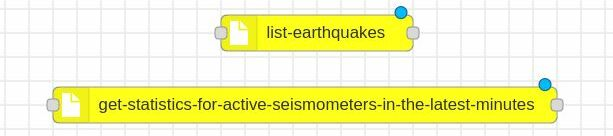
\includegraphics{relazione-tirocinio/Chapter-3/api-seismo.jpg}
    \caption{Nodi custom SeismoCloud per informazioni generali della rete}
    \label{fig:api-seismo-nodes}
\end{figure}


% ======================================= CHAPTER 4 ================================================
\chapter{Sicurezza e protezione dei dati}

\begin{itemize}
    \item Principio del privilegio minimo
    \item Dipendenze nodi SeismoCloud
    \item Controllo dell'input dell'utente
    \item Dati sensibili nelle variabili d'ambiente
    \item Nodi potenzialmente pericolosi
    \item Download ed inserimento di nodi esterni
    \item Download di librerie JS esterne (e.g. child\_process)
    \item Il nodo function ha accesso al context node, flow e global
    \item sandbox
\end{itemize}

\section{Sicurezza nella piattaforma Node-RED}

placeholder

\clearpage

\section{Ricerca ed analisi di vulnerabilità}

placeholder

\clearpage

\section{Risoluzione dei problemi}

placeholder

\clearpage


% ======================================= CHAPTER 5 ================================================
\chapter{Test, conclusioni e sviluppi futuri}

\section{Iterazioni dei Test}

Per una efficiente usabilità del sistema è assolutamente necessaria una parte accurata di test.
In questo caso sono stati coinvolti 7 utenti non esperti ed un esperto.
Le modalità di test sono due: in \textit{remoto} e \textit{dal vivo}. Questa scelta è motivata da vantaggi e svantaggi per una o per l'altra: da remoto si può controllare meglio tutta l'attività ``digitale" dell'utente, ad esempio i movimenti del cursore; con un test dal vivo invece si ha un maggior coinvolgimento da entrambe le parti, facendo così sentire l'utente più a suo agio e riuscendo a captare meglio le sue reazioni.
Sono state utilizzate diverse tecniche: \textbf{think aloud} (all'utente viene chiesto di pensare a voce alta ed esprimere tutte le emozioni, sensazioni e pensieri che ha durante tutta la durata del test), \textbf{cooperative evaluation} (utente e somministratore del test si pongono domande a vicenda ed esprimono i loro giudizi sull'esperienza d'uso), \textbf{post-task walkthrough} (finito il test, indipendentemente dal tipo effettuato, vengono poste delle domande per comprendere i risultati. Si hanno due opzioni 1) appena finito il test, dove l'utente ha ben chiare le sue opinioni, ma il somministratore non ha tempo di pensare alle domande, 2) il contrario del precedente) e \textbf{expert based} (un esperto revisiona l'interfaccia e da i suoi pareri su di essa) \cite{hcibook}.
Sono stati effettuate due sessioni di test con una revisione e correzione degli errori trovati appena effettuata la prima delle due.
I task scelti da svolgere per gli utenti erano quattro (con alcune variazioni durante i vari test per capire come reagivano gli utenti):

\begin{itemize}
    \item Difficoltà Livello 1: Prendere il valore Quake del sismometro ‘edotest’ e stamparlo nella console di debug.
    
    \begin{figure}[ht]
        \centering
        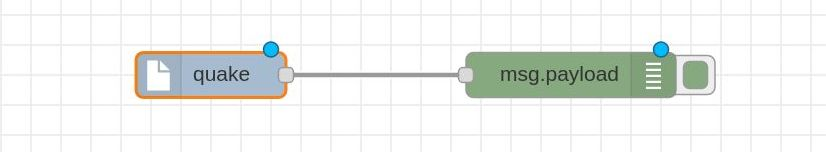
\includegraphics[width=1\textwidth]{relazione-tirocinio/Chapter-5/test-1.jpg}
        \label{fig:test1}
    \end{figure}
    
    \item Difficoltà Livello 2: Stampare tutte le informazioni del sismometro ‘edotest’ nella console di debug ogni volta che si riceve un segnale Quake.
    
    \begin{figure}[ht]
        \centering
        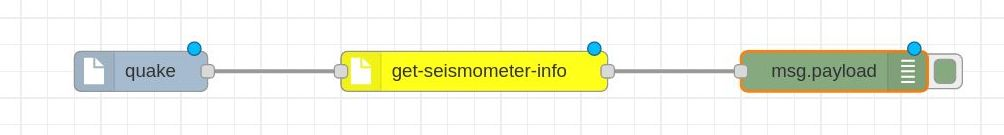
\includegraphics[width=1\textwidth]{relazione-tirocinio/Chapter-5/test-2.jpg}
        \label{fig:test1}
    \end{figure}
    
    \item Difficoltà Livello 3: Effettuare il reboot del sismometro ‘edotest’ ogni volta che la temperatura è maggiore di $x^{\circ}$C.
    
    \begin{figure}[ht]
        \centering
        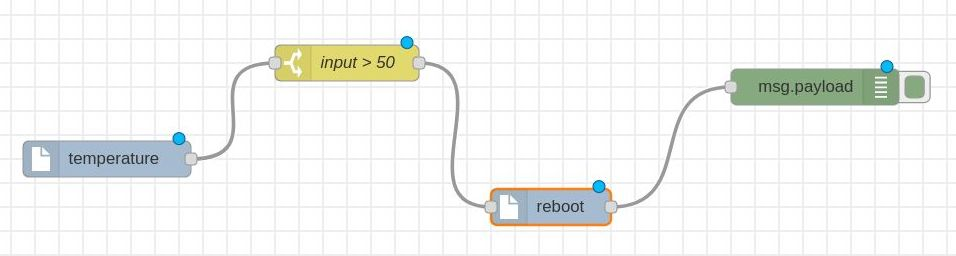
\includegraphics[width=1\textwidth]{relazione-tirocinio/Chapter-5/test-3.jpg}
        \label{fig:test1}
    \end{figure}
    
    \item Difficoltà livello 4: Prendere il valore Quake del sismometro ‘edotest’, applicare ad esso un template ( ad esempio ``\texttt{Quake: <payload>}" ) e stamparlo nella console di debug con le informazioni relative agli ultimi terremoti rilevati possibilmente rilevabili dal dispositivo.
    
    \begin{figure}[ht]
        \centering
        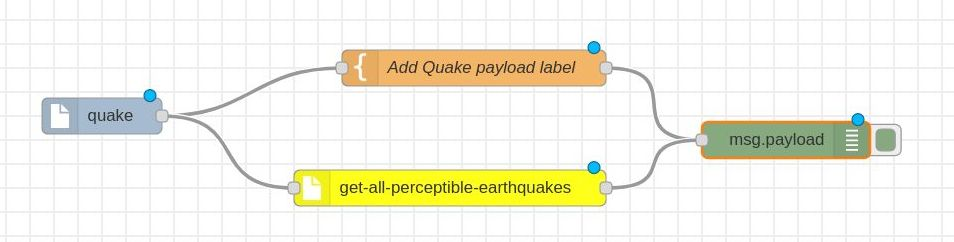
\includegraphics[width=1\textwidth]{relazione-tirocinio/Chapter-5/test-4.jpg}
        \label{fig:test1}
    \end{figure}
    
\end{itemize}

Effettuata la prima serie di test, con circa 15 test individuali sono stati evidenziati i seguenti problemi:

\begin{itemize}
    \item tasto di visualizzazione della console di debug non messo in risalto
    \item Prima clic destro su un nodo per la configurazione, solo dopo viene fatto un doppio clic
    \item Descrizione poco dettagliata dei valori del sismometro
    \item SeismometerAttributes è vago per indicare i dati relativi ai sismometri, meglio SeismometerData
\end{itemize}

Il primo problema nasce dal fatto che alcune funzionalità del sistema di End User Development per SeismoCloud non sono ancora state sviluppate. Perciò la disponibiltà di azioni è limitata a poche scelte. La console di debug una volta sviluppate o integrate (alcune funzionalità ``finali", quindi di notifica utente o nel senso di azione finale, sono già fornite dai vari produttori di servizi Web o da alcuni volenterosi sviluppatori Open Source: Telegram, Twitter, Email, integrazione con oggetti per smart-home) le funzionalità finali sarà solo uno strumento di utilità per controllare appunto se ci sono errori nei flussi progettati. Per questo motivo non è stato ritenuto un errore da risolvere.

Il secondo problema è stato rilevato maggiormente durante i test da remoto, dove il controllo del cursore dell'utente è più intenso. Quando un utente doveva selezionare un nodo per configurare le impostazioni di base (nome del nodo, sismometro selezionato) 4 dei 7 utenti hanno in prima battuta provato un clic destro sul nodo, che non ha nessun effetto, e poi in seconda battuta un doppio clic sinistro, che è appunto l'azione corretta.

La terza criticità era la descrizione di alcuni nodi, per esempio, uno di questi era il nodo \textbf{BSSID}. Questo termine indica l'indirizzo MAC di un punto di accesso alla rete dove il sismometro si connette.
Il problema è stato rilevato chiedendo (durante la tipologia di test \textit{cooperative evaluation}) agli utenti se, una volta configurato il nodo, avessero capito che tipologia di dati stavano usando, o quanto meno sapessero dare una spiegazione sommaria.
Tutti gli utenti non competenti hanno risposto che il nodo restituisce un valore in output, ma che non avevano capito minimamente la tipologia di dato.

L'ultimo problema è stato rilevato dal somministratore dei test, dato che il titolo ``SeismometerAttributes" non era adatto a descrivere in modo comprensibile le funzionalità coinvolte e soprattutto non entrava nel box ad esso dedicato.

La seconda sessione di test è stata effettuata dopo aver parzialmente risolto i problemi della prima. È stata aggiunta una descrizione molto più dettagliata per tutti i nodi di cui risultava ambiguo il significato ed è stato modificato il nome ``SeismometerAttributes" con ``SeismometerData". Le modifiche sono state sottoposte ai test e hanno avuto esito positivo.

Tutti gli utenti hanno compreso come i nodi devono essere collegati per formare un flusso, prendendo e rilasciando i nodi dalla palette dei nodi allo spazio di lavoro. Data la differenziazione in categorie per argomenti differenti (e colorati in modo differente), cercare un singolo nodo sulla palette è risultato un facile compito. Tutti gli utenti hanno completato i compiti di basso e medio livello senza problemi significativi, anche se ci è voluto più tempo del previsto per i compiti di alta difficoltà.

\section{Conclusioni}

Dai risultati che sono stati ottenuti si sta procedendo nella giusta direzione.
Abbiamo visto come poter progettare ed implementare un sistema di End User Development \textbf{sicuro, efficiente e facilmente usabile}.
Sono stati trovati i problemi più evidenti in sicurezza ed in usabilità; è stata applicata una soluzione efficace per alcuni, per altri è definito il metodo di risoluzione.
Come si nota dalle implementazioni tecniche apportate descritte nel capitolo 3 e dai test svolti definiti in questo capitolo, l'interfaccia risulta usabile e richiede la minima configurazione dell'utente per programmare anche azioni complesse senza avere una conoscenza tecnica né di programmazione, né di protocolli di rete.
L'applicativo è stabile, è stato testato più volte con gli utenti ed internamente nel team di sviluppo.
Come abbiamo visto nel capitolo 4 è anche sicuro e i dati della rete di sismometri e le informazioni personali degli utenti SeismoCloud rimangono protetti.
È stata creata una piattaforma che sarà utilizzata come base con le funzionalità necessarie ad interfacciarsi con il sistema ed i vari dispositivi connessi.
Si continuerà ad ascoltare gli utenti SeismoCloud ricevendo feedback utili e proposte di servizi cercando di far rimanere il sistema comprensibile, sicuro ed usabile.
Nel prossimo paragrafo vengono poi espressi alcuni percorsi da seguire per aggiungere interessanti funzionalità e continuare ad elevare l'utilità di questo sistema.
\clearpage

\section{Sviluppi futuri}

\subsection{Integrazione social network}

L'introduzione di azioni che utilizzano le API di social network o funzioni di notifica è molto utile. In particolare, esiste già un modulo NPM pronto e maturo (Versione 8.6.4) per Telegram \cite{telegram-node}, per Twitter \cite{twitter-node} e per Facebook \cite{facebook-node}.
Sono molto utili per condividere dati, ma soprattutto per notificare ad un bacino molto ampio di utenza facile da raggiungere Earthquake Early Warning. In più, per quanto riguarda Twitter e Facebook, non è nemmeno necessario conoscere dati dei destinatari del messaggio, basta condividere un messaggio automatico con le informazioni utili. Ancora più utile è la possibilità di localizzare il proprio Tweet (o post Facebook) tramite la localizzazione GPS per una più rapida ed efficace diffusione dell stesso in aree interessate all'evento sismico.
L'INGV ha avviato un servizio simile, questo un Tweet di esempio(\href{https://twitter.com/ingvterremoti/status/1259681114920230912}{https://twitter.com/ingvterremoti/status/1259681114920230912}):
\begin{figure}[ht]
    \centering
    
\includegraphics[width=1\textwidth]{relazione-tirocinio/Chapter-5/tweetINGV.jpg}
    \label{fig:tweetINGV}
\end{figure}

\subsection{Integrazione dispositivi IoT per smart-home}

Come è stato introdotto nel capitolo 2.1, una funzionalità interessante sarebbe l'integrazione con dispositivi per una smart-home. Anche qui dato l'alto contributo della community esistono moduli pronti all'uso (necessaria configurazione). Ad esempio integrazione con Alexa \cite{alexa} e Google Home \cite{google-home}.
Oltre ai soliti dispositivi smart (luci, elettrodomestici, TV...) l'utente ha completa libertà (privilegiando l'usabilità e la sicurezza) di creare da sé programmi software che si interfacciano con dispositivi hardware creati personalmente. Ad esempio, programmare un GPIO (General Purpose Input/Output) ad emettere un segnale quando avviene una certa condizione. Quest'ultimo poi potrà essere utilizzato per interfacciarsi con dispositivi che hanno bisogno di essere spenti o accesi in determinate condizioni di sicurezza (generatore elettrico, valvola del gas), dato che il GPIO ha solo due stati.

\subsection{Ottimizzazione delle prestazioni tramite la condivisione di un solo client MQTT}

Un ristretto limite prestazionale è dato dall'utilizzo di tanti client MQTT quanti sono i nodi presenti nel workspace. La libreria MQTT utilizzata offre la disponibilità di assegnare un identificativo univoco per ogni client.
L'attuale implementazione istanzia un client MQTT (con un identificativo randomico con il formato 
\begin{lstlisting}[language=Javascript]
clientId: 'mqttjs_' + Math.random().toString(16).substr(2, 8))
\end{lstlisting}
ogni volta che viene creato un nodo, e viene distrutto quando il nodo viene cancellato dal workspace.
In generale, data la brevità dei messaggi trasferiti e l'implementazione orientata all'efficienza del protocollo MQTT, l'applicativo non ne risente molto; ma con il crescere dei gruppi, degli utenti e quindi dei dispositivi coinvolti si potrebbero aver problemi di scalabilità, per questo un unico client condiviso con i nodi del gruppo (o flusso, dipende dalle connessione simultanee possibili) potrebbe aiutare l'efficienza del sistema.
Inoltre, con le variabili a differente scope (Node, Flow e Global definite nel paragrafo 2.2) è possibile condividere in modo facile lo stesso client per azioni differenti.

\clearpage

\refstepcounter{chapter}

\chapter*{Ringraziamenti}

\cleardoublepage

\refstepcounter{chapter}

% ======================================= BIBLIOGRAPHY ================================================
\begin{thebibliography}{9}

\bibitem{terra}
  \textbf{The inner structure of the Earth}.\\
  \href{http://sci.fgt.bme.hu/~volgyesi/gravity/ppfold.pdf}{http://sci.fgt.bme.hu/~volgyesi/gravity/ppfold.pdf}\\
  1982, L.Volgeyesi, M. Moser

\bibitem{measure}
  \textbf{Earthquake Magnitude, Energy Release, and Shaking Intensity}.\\
  \href{https://www.usgs.gov/natural-hazards/earthquake-hazards/science/earthquake-magnitude-energy-release-and-shaking-intensity}{https://www.usgs.gov/natural-hazards/earthquake-hazards/science/earthquake-magnitude-energy-release-and-shaking-intensity}

\bibitem{ingv}
  \textbf{Istituto Nazionale di Geologia e Vulcanologia}.
  \href{http://ingv.it}{http://ingv.it}

\bibitem{ottimizzazione}
  \textbf{Ottimizzazione delle risorse nell’uso di servizi in background in SeismoCloud per Android}, 2017, Enrico Bassetti 
  \href{https://github.com/Enrico204/bachelor-degree-thesis}{https://github.com/Enrico204/bachelor-degree-thesis}

\bibitem{berkeleyfaq}
  \textbf{Seismo Berkeley Lab FAQ}.
  \href{http://seismo.berkeley.edu/outreach/faq.html}{http://seismo.berkeley.edu/outreach/faq.html}

\bibitem{rest}
  \textbf{REST API documentation}.
  \href{https://restfulapi.net/}{https://restfulapi.net/}

\bibitem{wikieud}
  \textbf{Wikipedia - End User Development}.\\
  \href{https://en.wikipedia.org/wiki/End-user_development}{https://en.wikipedia.org/wiki/End-user\_development}

\bibitem{MathWorks}
  \textbf{Publish MQTT messages and subscribe to message topics}.\\
  \href{https://www.mathworks.com/help/supportpkg/raspberrypi/ref/publish-and-subscribe-to-mqtt-messages.html}{https://www.mathworks.com/help/supportpkg/raspberrypi/ref/publish-and-subscribe-to-mqtt-messages.html}

\bibitem{noderedwiki}
  \textbf{Node-RED Wiki}.
  \href{https://github.com/node-red/node-red/wiki}{https://github.com/node-red/node-red/wiki}

\bibitem{wikidocker}
  \textbf{Wikipedia - Docker}.
  \href{https://it.wikipedia.org/wiki/Docker/}{https://it.wikipedia.org/wiki/Docker}

\bibitem{docker-portability}
  \textbf{What does Docker technology add to just plain lxc}.\\
  \href{https://docs.docker.com/engine/faq/#what-does-docker-technology-add-to-just-plain-lxc}{https://docs.docker.com/engine/faq/\#what-does-docker-technology-add-to-just-plain-lxc}

\bibitem{aboutstoragedrivers}
  \textbf{Docker docs - About storage drivers}.\\
  \href{https://docs.docker.com/storage/storagedriver/}{https://docs.docker.com/storage/storagedriver/}

\bibitem{dockervsvm2}
    \textbf{How is Docker different from a Virtual Machine}
    \\
    \href{https://stackoverflow.com/questions/16047306/how-is-docker-different-from-a-virtual-machine}{https://stackoverflow.com/questions/16047306/how-is-docker-different-from-a-virtual-machine}

\bibitem{dockervsvm}
    \textbf{Performance Evaluation of Docker Container and Virtual Machine}
    \\
    \href{https://www.sciencedirect.com/science/article/pii/S1877050920311315}{https://www.sciencedirect.com/science/article/pii/S1877050920311315},
    \\
    2019, Amit M Potdar, Narayan D G, Shivaraj Kengond, Mohammed Moin Mulla.

\bibitem{dockerfilesbestpractices}
    \textbf{Best practices for writing Dockerfiles}
    \\
    \href{https://docs.docker.com/develop/develop-images/dockerfile_best-practices/}{https://docs.docker.com/develop/develop-images/dockerfile\_best-practices/}

\bibitem{hcibook}
    \textbf{Human Computer Interaction Book - Evaluation techniques}
    \\
    \href{https://www.hcibook.com/e3-docs/slides/notes-pdf/e3-chap-09-6up.pdf}{https://www.hcibook.com/e3-docs/slides/notes-pdf/e3-chap-09-6up.pdf}
    
\bibitem{noderedconfig}
    \textbf{Node-RED Docs: Configuration }
    \\
    \href{https://nodered.org/docs/user-guide/runtime/configuration}{https://nodered.org/docs/user-guide/runtime/configuration}

\bibitem{mqttjs}
    \textbf{MQTT.js Docs}
    \\
    \href{https://github.com/mqttjs/MQTT.js/wiki}{https://github.com/mqttjs/MQTT.js/wiki}
    
\bibitem{securingNode-RED}
    \textbf{Securing IoT Apps in Node-RED | University of Gothenburg}
    \\
    \href{https://odr.chalmers.se/bitstream/20.500.12380/300759/1/CSE\%2020-06\%20Olsson\%20ODR.pdf}{https://odr.chalmers.se/bitstream/20.500.12380/300759/1/CSE\%2020-06\%20Olsson\%20ODR.pdf}
    \\
    2020, Lars Eric Olsson.
    
\bibitem{telegram-node}
    \textbf{Node-RED Library | Telegram node}
    \\
    \href{https://flows.nodered.org/node/node-red-contrib-telegrambot}{https://flows.nodered.org/node/node-red-contrib-telegrambot}.
    \\
    2020, [Online, acceduto il 16/09/2020]
    
\bibitem{twitter-node}
    \textbf{Node-RED Library | Twitter node}
    \\
    \href{https://flows.nodered.org/node/node-red-node-twitter}{https://flows.nodered.org/node/node-red-node-twitter}.
    \\
    2020, [Online, acceduto il 16/09/2020]
    
\bibitem{facebook-node}
    \textbf{Node-RED Library | Facebook node}
    \\
    \href{https://flows.nodered.org/node/node-red-contrib-facebook}{https://flows.nodered.org/node/node-red-contrib-facebook}.
    \\
    2020, [Online, acceduto il 16/09/2020]

\bibitem{alexa}
    \textbf{Node-RED Library | Alexa Assistant}
    \\
    \href{https://flows.nodered.org/node/node-red-contrib-alexa-smart-home}{https://flows.nodered.org/node/node-red-contrib-alexa-smart-home}.
    \\
    2020, [Online, acceduto il 16/09/2020]

\bibitem{google-home}
    \textbf{Node-RED Library | Google Home Assistant}
    \\
    \href{https://flows.nodered.org/node/node-red-contrib-googlehome}{https://flows.nodered.org/node/node-red-contrib-googlehome}.
    \\
    2020, [Online, acceduto il 16/09/2020]

\end{thebibliography}

\end{document}